\documentclass[11pt,a4paper]{article}

\usepackage{fontspec}
\setmainfont{Latin Modern Roman}
\setsansfont{Latin Modern Sans}
\setmonofont{Latin Modern Mono}
\usepackage{polyglossia}
\setdefaultlanguage{vietnamese}
\usepackage[margin=2.15cm]{geometry}
\usepackage{graphicx}
\usepackage{booktabs}
\usepackage{array}
\usepackage{longtable}
\usepackage{caption}
\usepackage{subcaption}
\usepackage{amsmath,amssymb}
\usepackage{hyperref}
\usepackage{xurl}
\usepackage{xcolor}
\usepackage{enumitem}
\usepackage{float}
\usepackage{microtype}
\usepackage{seqsplit}
\usepackage{tikz}
\usetikzlibrary{arrows.meta,positioning,shapes.geometric}

\graphicspath{{figures/}}
\hypersetup{colorlinks=true,linkcolor=black,citecolor=black,urlcolor=blue}
\AtBeginDocument{%
    \renewcommand{\contentsname}{Mục lục}%
    \renewcommand{\listfigurename}{Danh mục hình}%
    \renewcommand{\listtablename}{Danh mục bảng}%
}
\setlist{nosep,leftmargin=1.4em}
\captionsetup{font=small,labelfont=bf}
\newcommand{\unitpm}{$\mu$g/m$^3$}

\title{\textbf{DỰ BÁO ĐA CHÂN TRỜI NỒNG ĐỘ PM2.5\\TỪ 1 ĐẾN 24 GIỜ TẠI VIỆT NAM}\\[4pt]
\large Đồ án môn Xây dựng và Triển khai Hệ thống Học máy Ứng dụng\\[8pt]
\small Mã nguồn: \url{https://github.com/kimngoc280105/aqi-vietnam}}
\author{Nhóm 11\\[4pt]
\begin{tabular}{ll}
Trần Kim Ngọc & 23120062\\
Nguyễn Thành Nguyên & 23120063\\
Nguyễn Mạnh Thắng & 23120084\\
Trần Đình Luân & 23120059\\
Nguyễn Thiện Nhân & 23120064
\end{tabular}}
\date{Năm học 2025--2026}

\begin{document}
\maketitle
\tableofcontents
\clearpage
\vspace*{0.3cm}
\phantomsection
\section*{Danh mục hình}
\addcontentsline{toc}{section}{Danh mục hình}
\makeatletter
\@starttoc{lof}
\makeatother
\clearpage
\vspace*{0.3cm}
\phantomsection
\section*{Danh mục bảng}
\addcontentsline{toc}{section}{Danh mục bảng}
\makeatletter
\@starttoc{lot}
\makeatother
\clearpage

\section*{Thông tin nhóm và phân công công việc}
\addcontentsline{toc}{section}{Thông tin nhóm và phân công công việc}
\begin{table}[H]
\centering\small
\caption{Phân công công việc của nhóm}
\label{tab:roles}
\begin{tabular}{p{3.5cm}p{1.8cm}p{9.2cm}}
\toprule
Họ và tên & MSSV & Phân công công việc\\
\midrule
Trần Kim Ngọc & 23120062 & Xác định bài toán, xây dựng quy trình crawl Open-Meteo, kiểm tra dữ liệu, biên tập báo cáo và slide.\\
Nguyễn Thành Nguyên & 23120063 & Làm sạch dữ liệu, EDA, thiết kế đặc trưng lag, rolling, chu kỳ và đặc trưng tương tác.\\
Nguyễn Mạnh Thắng & 23120084 & Xây dựng SARIMAX đa chân trời, giao thức temporal split và phân tích lỗi theo thời gian.\\
Trần Đình Luân & 23120059 & Xây dựng LSTM Sequence-to-Vector, theo dõi learning curve và kiểm soát overfitting.\\
Nguyễn Thiện Nhân & 23120064 & Xây dựng XGBoost Direct Multi-Horizon, FastAPI, React, Docker và tích hợp model vào web.\\
\bottomrule
\end{tabular}
\end{table}

\section{Chương 1: Giới thiệu}
\subsection{Phân tích vấn đề}
PM2.5 là bụi mịn có khả năng đi sâu vào hệ hô hấp và liên quan đến nhiều rủi ro sức khỏe. Tại Hà Nội, TP.HCM và Đà Nẵng, nồng độ PM2.5 biến động theo giờ, theo mùa, điều kiện khuếch tán khí quyển và nguồn phát thải. Một dự báo duy nhất tại $t+24$ chỉ trả lời trạng thái cuối ngày, trong khi người dùng cần biết diễn biến từng giờ để quyết định thời gian đi lại, tập luyện hoặc hạn chế tiếp xúc.

Trong bối cảnh Việt Nam, ba thành phố đại diện cho các chế độ khí tượng và phát thải khác nhau. Hà Nội chịu mùa đông lạnh, điều kiện nghịch nhiệt và những giai đoạn tích tụ kéo dài; TP.HCM có khí hậu nóng ẩm và hai mùa rõ; Đà Nẵng chịu ảnh hưởng mạnh của biển và gió. Do đó, một mô hình dùng chung phải vừa học quy luật thời gian phổ quát vừa giữ được khác biệt địa lý. Đây không chỉ là bài toán tối ưu một chỉ số trung bình: sai số cần được phân rã theo thành phố, thời điểm và độ dài chân trời dự báo để tránh che khuất vùng hoạt động kém.

Bài toán còn có ba khó khăn kỹ thuật. Thứ nhất, các target tương lai chồng lấn mạnh giữa hai origin liên tiếp, nên chia ngẫu nhiên sẽ gây rò rỉ thời gian. Thứ hai, phân phối PM2.5 lệch phải khiến một số ít đỉnh ô nhiễm đóng góp lớn vào RMSE. Thứ ba, sai số thường tăng theo horizon vì thông tin quan sát tại $t$ dần mất giá trị. Thiết kế thực nghiệm vì vậy phải tôn trọng thứ tự thời gian, giữ các đỉnh hợp lệ và báo cáo hiệu năng theo từng $t+h$.

Đồ án mới giải bài toán \textbf{hồi quy đa đầu ra}: tại thời điểm $t$, mô hình dự báo đồng thời 24 giá trị PM2.5 trong tương lai,
\begin{equation}
\hat{\mathbf y}_t=[\widehat{PM}_{t+1},\widehat{PM}_{t+2},\ldots,\widehat{PM}_{t+24}].
\end{equation}
Target vẫn là PM2.5 liên tục, không phải AQI và không phải PM2.5 hiện tại. Khác với phiên bản cũ chỉ dự báo $t+24$, phiên bản này cho phép người dùng chọn bất kỳ horizon từ 1 đến 24 giờ.

\subsection{Mục tiêu và đóng góp}
\begin{itemize}
\item Thu thập và xử lý dữ liệu theo giờ trong bối cảnh ba thành phố Việt Nam.
\item Tạo 24 target đúng timestamp và xây dựng đặc trưng chỉ từ thông tin tại $t$ hoặc quá khứ.
\item So sánh SARIMAX, XGBoost và LSTM trên cùng temporal split; kiểm tra độ ổn định bằng năm khối Validation liên tiếp.
\item Đánh giá RMSE, MAE, R$^2$, bias, sai số theo horizon và thành phố; dùng dải PM2.5 hậu xử lý để phân tích lỗi.
\item Hiệu chỉnh khoảng conformal 90\% theo thành phố và horizon.
\item Tích hợp XGBoost Direct Multi-Horizon vào FastAPI và React để dự báo tự động hoặc nhập kịch bản.
\end{itemize}

Các nhiệm vụ được phân công theo Bảng~\ref{tab:roles}, nhưng mọi thành viên cùng kiểm tra giao thức dữ liệu, kết quả Test và tính nhất quán giữa notebook, artifact triển khai và tài liệu. Cách tổ chức này giảm nguy cơ mỗi thành phần sử dụng một định nghĩa target hoặc một phiên bản dữ liệu khác nhau.

\subsection{Tổng quan phương pháp}
Quy trình end-to-end gồm sáu khối. Dữ liệu không khí và khí tượng được thu thập theo giờ; sau kiểm tra schema, thời gian và giá trị vật lý, dữ liệu được làm sạch riêng theo thành phố. Feature engineering tạo các biến lịch sử, rolling, chu kỳ và tương tác nhưng chỉ từ thông tin có sẵn tại origin. Tiếp theo, 24 target được ghép bằng timestamp chính xác và chia theo thời gian thành Train, Validation và Test. Ba họ mô hình đại diện cho thống kê tuyến tính, boosting cây và học sâu chuỗi được huấn luyện trên cùng giao thức. Model được chọn bằng năm khối Validation liên tiếp, sau đó mới đánh giá một lần trên Test. Cuối cùng, artifact thắng được đóng gói trong FastAPI và phục vụ giao diện React.

Thiết kế ba họ mô hình giúp việc so sánh có ý nghĩa hơn so với chỉ thay đổi siêu tham số trong cùng một thuật toán. SARIMAX kiểm tra mức hiệu quả của cấu trúc tự hồi quy tuyến tính; XGBoost kiểm tra quan hệ phi tuyến trên feature dạng bảng; LSTM kiểm tra khả năng học biểu diễn trực tiếp từ cửa sổ chuỗi. Việc Test bị khóa trong lựa chọn model tuân theo nguyên tắc đánh giá out-of-sample cho chuỗi thời gian~\cite{tashman}.

\subsection{Lý do giữ PM2.5 làm target}
AQI được giữ như thông tin tham chiếu trong EDA, nhưng model học trực tiếp PM2.5 vì đại lượng này giữ biên độ vật lý và phù hợp với mục tiêu cảnh báo bụi mịn. Nếu đổi sang phân loại AQI, các giá trị rất khác nhau trong cùng một dải sẽ bị xem như tương đương, làm mất thông tin biên độ và gây gián đoạn nhân tạo tại ngưỡng lớp. Dự báo PM2.5 liên tục vẫn cho phép ánh xạ sang dải cảnh báo ở bước hậu xử lý. Hình~\ref{fig:pivot-dist} cho thấy PM2.5 lệch phải rõ và có các đỉnh hiếm; Hình~\ref{fig:pivot-time} cho thấy cấu trúc theo giờ, theo thời gian và tự tương quan.

\begin{figure}[H]
\centering
\begin{subfigure}{0.49\linewidth}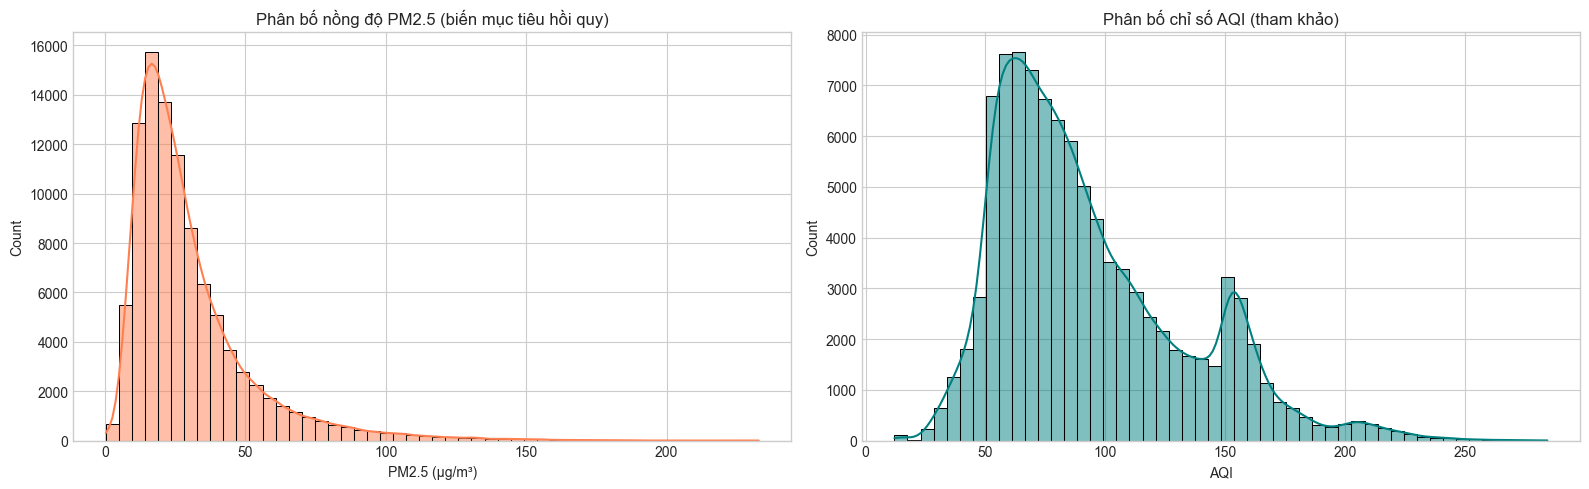
\includegraphics[width=\linewidth]{eda_pm25_aqi_distributions.png}\caption{Phân phối PM2.5 và AQI}\end{subfigure}
\begin{subfigure}{0.49\linewidth}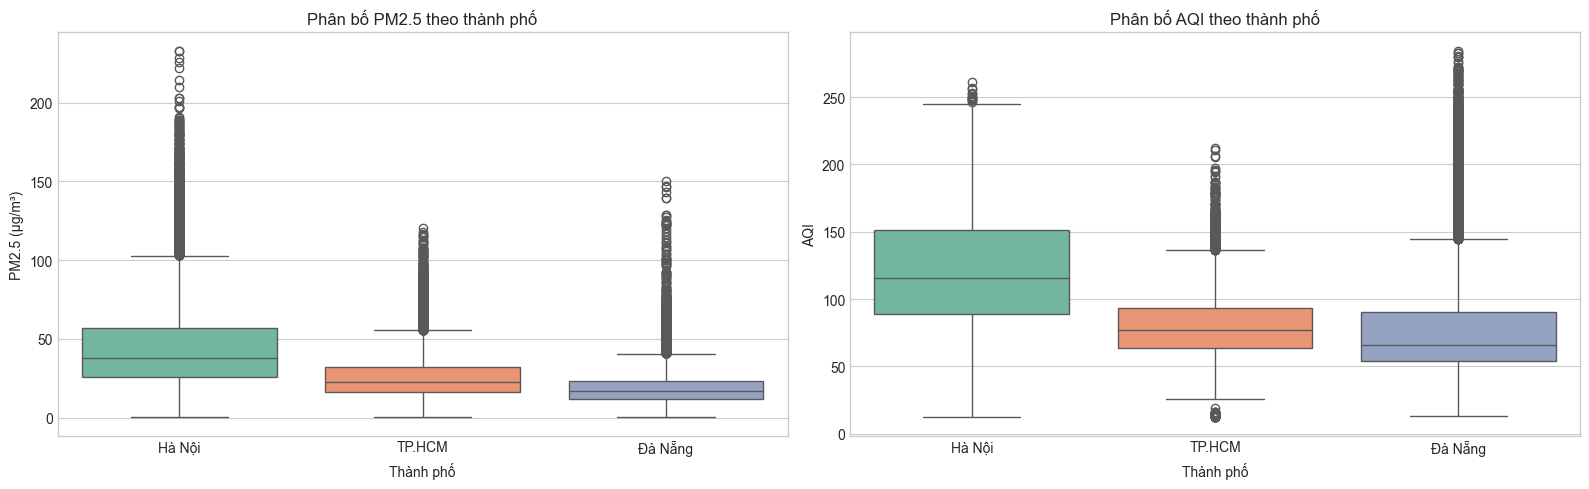
\includegraphics[width=\linewidth]{eda_pm25_aqi_boxplots.png}\caption{Độ phân tán và cực trị}\end{subfigure}
\caption{So sánh PM2.5 và AQI phục vụ lựa chọn target; model cuối vẫn là hồi quy PM2.5.}
\label{fig:pivot-dist}
\end{figure}

\begin{figure}[H]
\centering
\begin{subfigure}{0.32\linewidth}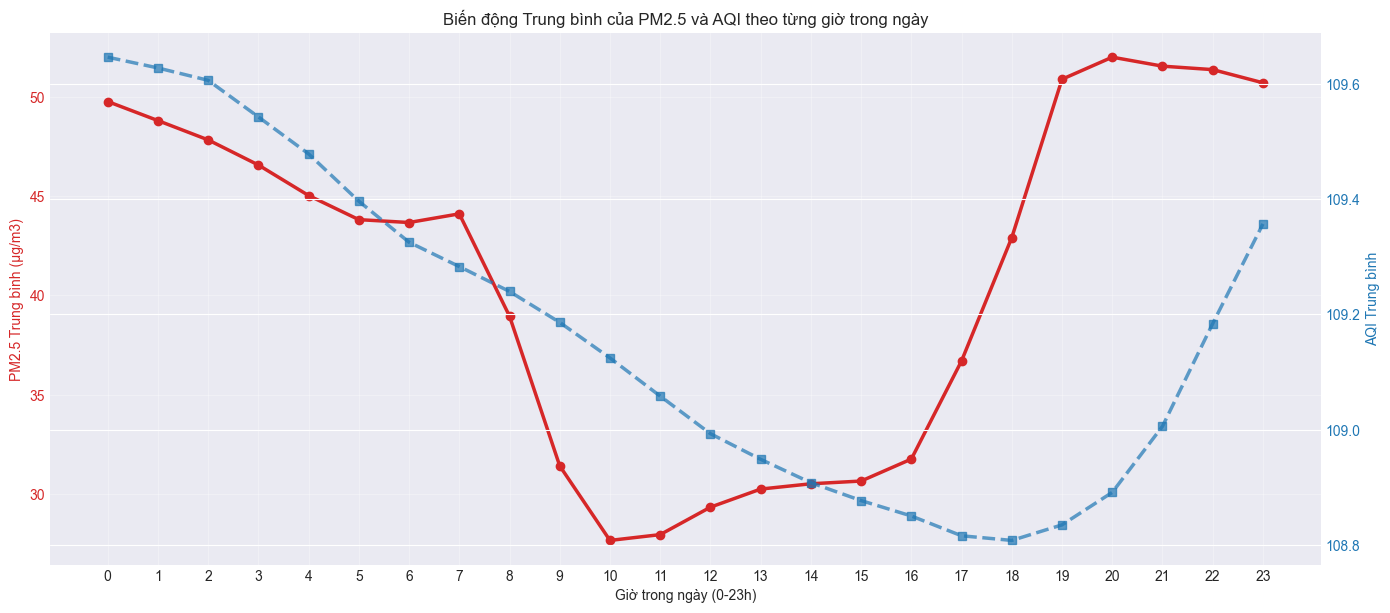
\includegraphics[width=\linewidth]{pm25_aqi_hourly_profile.png}\caption{Hồ sơ theo giờ}\end{subfigure}
\begin{subfigure}{0.32\linewidth}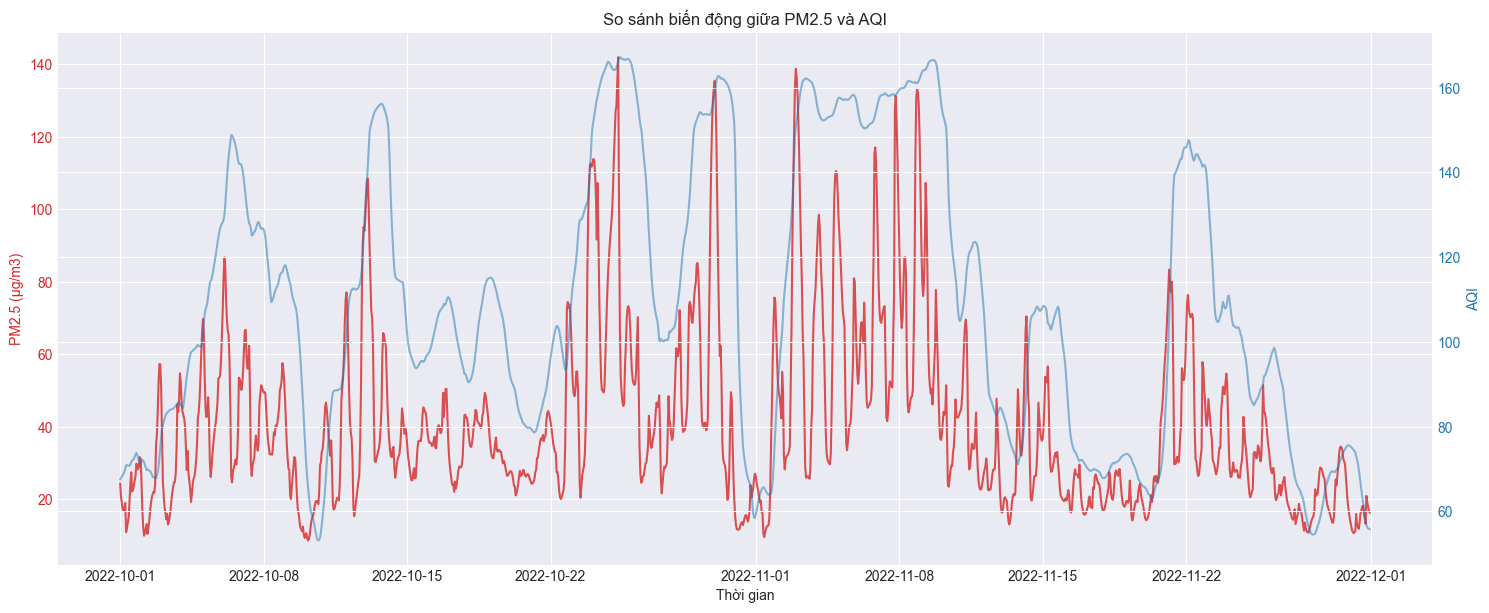
\includegraphics[width=\linewidth]{pm25_aqi_timeseries.png}\caption{Chuỗi thời gian}\end{subfigure}
\begin{subfigure}{0.32\linewidth}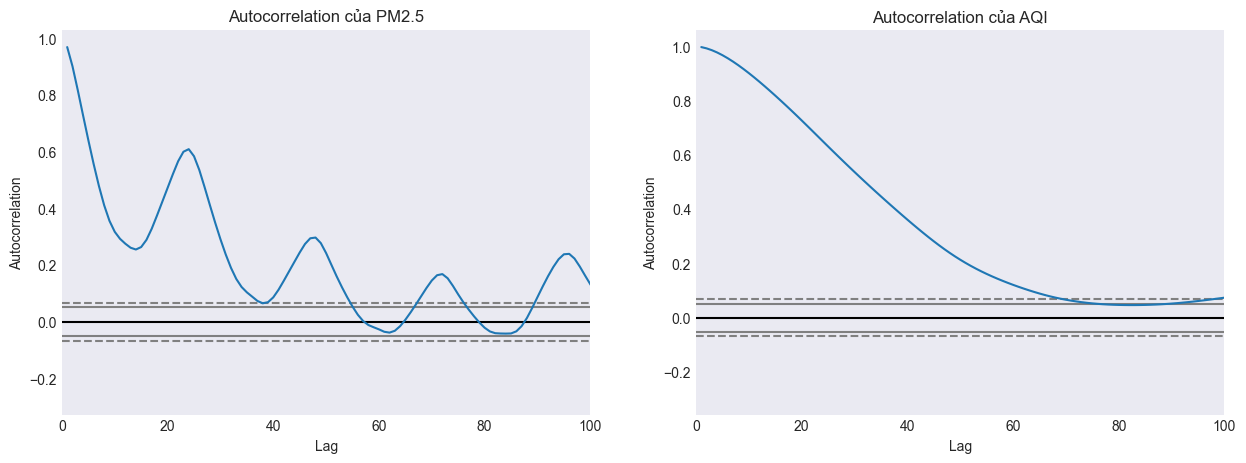
\includegraphics[width=\linewidth]{pm25_aqi_autocorrelation.png}\caption{Tự tương quan}\end{subfigure}
\caption{Các góc nhìn thời gian cho thấy PM2.5 có cấu trúc ngắn hạn và chu kỳ cần được mô hình hóa.}
\label{fig:pivot-time}
\end{figure}

\section{Chương 2: Thu thập và Phân tích Dữ liệu}
\subsection{Nguồn và phương pháp thu thập}
Dữ liệu được crawl theo giờ từ Open-Meteo Air Quality API và Historical Weather API~\cite{openmeteo}. Thành phần không khí gồm PM2.5, PM10, O$_3$, NO$_2$, SO$_2$, CO; thành phần khí tượng gồm nhiệt độ, độ ẩm, tốc độ và hướng gió, mưa, áp suất, mây. Mỗi thành phố được đại diện bởi một điểm lưới CAMS gần trung tâm. Đây là dữ liệu lưới mô hình khí quyển, không phải số đo trạm mặt đất và không được diễn giải ở cấp quận.

Script thu thập gửi truy vấn theo tọa độ, khoảng ngày và danh sách biến, sau đó chuẩn hóa phản hồi về bảng theo giờ. Thời gian được chuyển về cùng chuẩn trước khi nối dữ liệu chất lượng không khí với khí tượng bằng khóa thành phố--timestamp. Dữ liệu thô được giữ riêng với dữ liệu đã xử lý để có thể truy vết; notebook EDA chỉ đọc bản đã hợp nhất, còn notebook chuẩn bị model tạo target và feature trong thư mục model. Quy trình không tự sinh giá trị quan trắc thay thế cho API.

Sau mỗi lần crawl, nhóm kiểm tra số giờ kỳ vọng, tính đơn điệu của timestamp, số bản ghi trùng, miền giá trị và tỷ lệ thiếu. Các kiểm tra này quan trọng vì API có thể trả về đoạn thời gian ngắn hơn yêu cầu hoặc cập nhật lại dữ liệu lịch sử. Phạm vi cuối cùng được trình bày ở Bảng~\ref{tab:scope}. Hạn chế nguồn phải được hiểu đúng: một điểm lưới có ích cho dự báo ở quy mô thành phố nhưng không đủ để kết luận chất lượng không khí tại từng quận hoặc vị trí đường phố.

\begin{table}[H]
\centering\small
\caption{Phạm vi dữ liệu đầu vào}
\label{tab:scope}
\begin{tabular}{ll}
\toprule
Thuộc tính & Giá trị\\
\midrule
Khu vực & Hà Nội, TP.HCM, Đà Nẵng\\
Khoảng thời gian & 05/08/2022 đến 09/05/2026\\
Tần suất & 1 giờ\\
Quy mô & 98.907 dòng, 76 cột sau tạo đặc trưng\\
Trùng city--datetime & 0 dòng\\
Nguồn & Open-Meteo / CAMS Global\\
\bottomrule
\end{tabular}
\end{table}

\subsection{EDA và chất lượng dữ liệu}
EDA được thực hiện trước khi quyết định cách làm sạch và tạo đặc trưng. Phân phối PM2.5 lệch phải ở cả ba thành phố. Hà Nội có mức trung bình và độ biến động lớn nhất; Đà Nẵng thấp hơn nhưng vẫn xuất hiện một số cực trị. Hình~\ref{fig:eda-distributions} cho thấy các biến đầu vào khác nhau rõ về thang đo và độ lệch; Hình~\ref{fig:eda-correlation} cho thấy PM2.5 tương quan cao với PM10, trong khi quan hệ khí tượng yếu hơn và có thể phi tuyến.

\begin{figure}[H]
\centering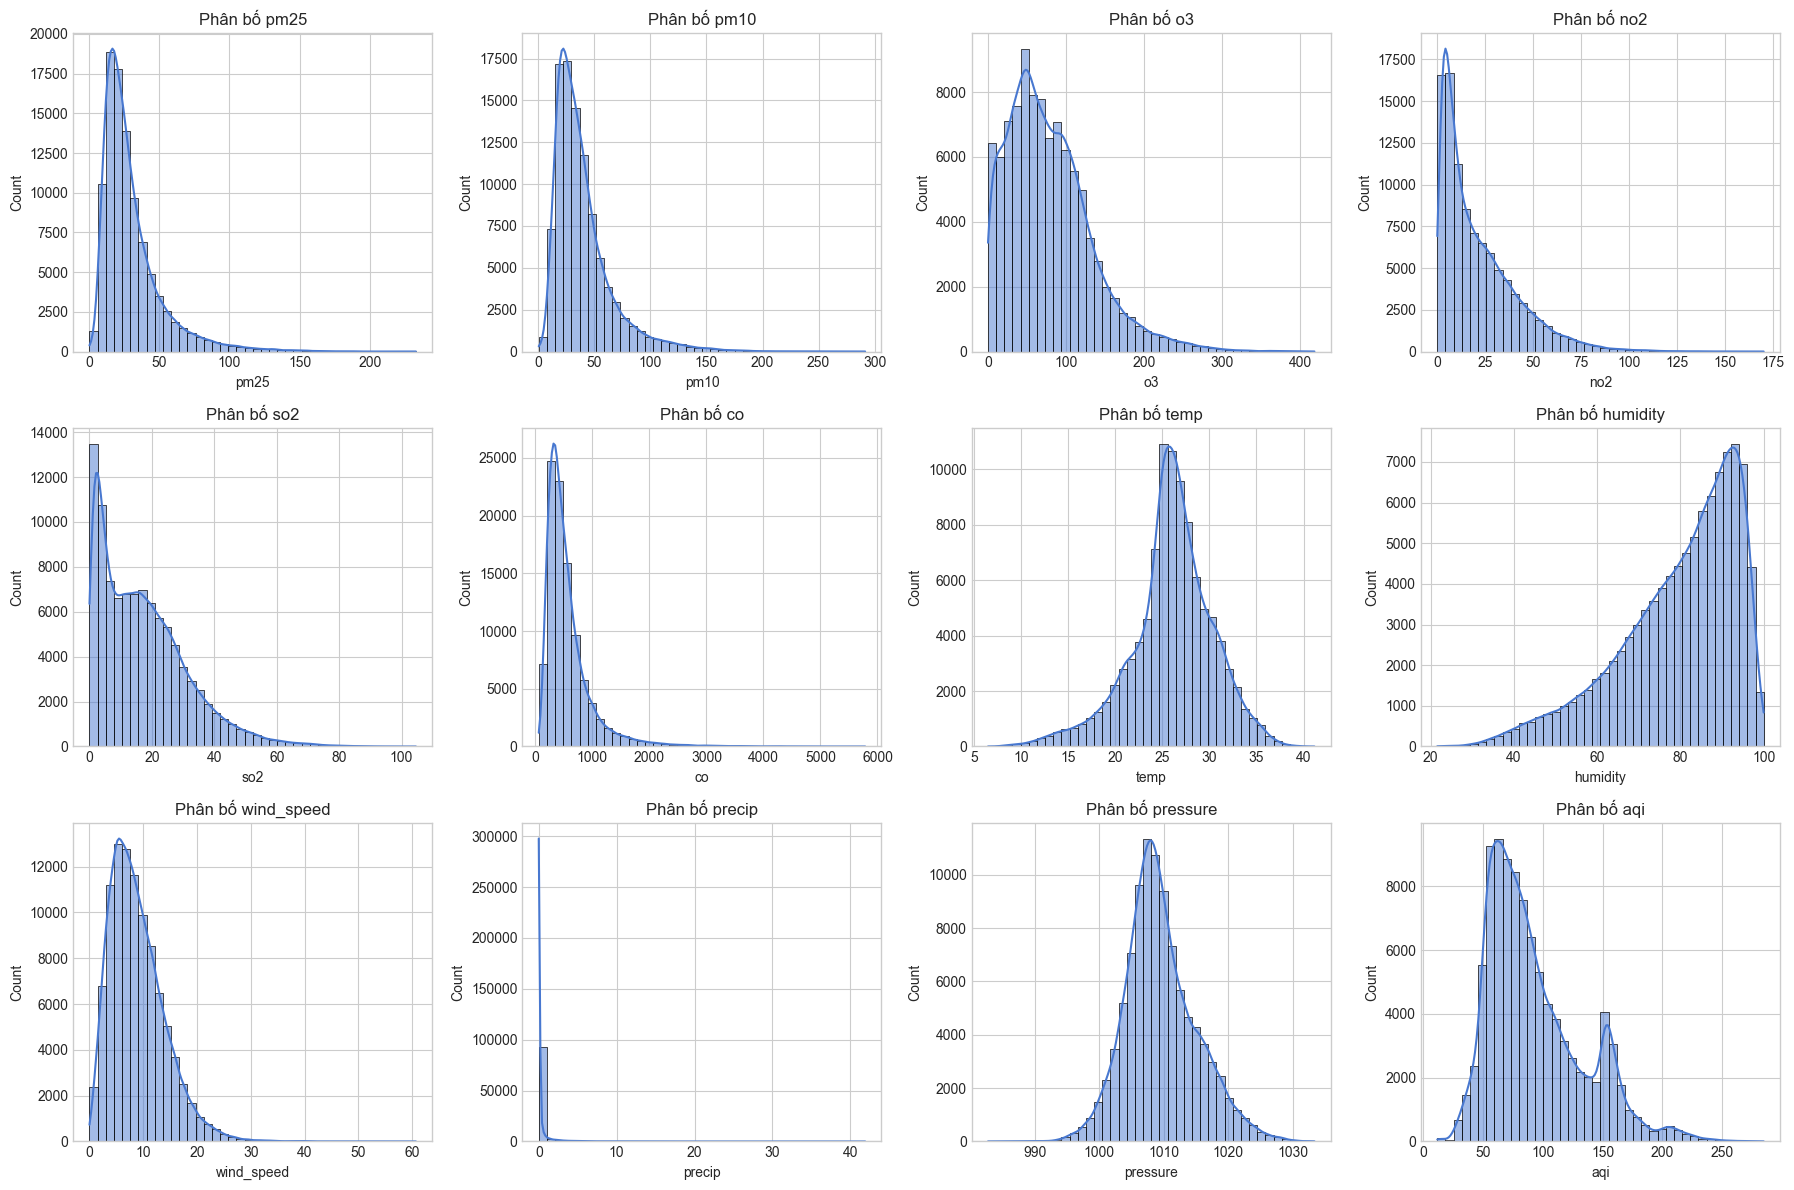
\includegraphics[width=0.92\linewidth]{eda_feature_distributions.png}
\caption{Phân phối các biến ô nhiễm và khí tượng trong bước EDA.}
\label{fig:eda-distributions}
\end{figure}

\begin{figure}[H]
\centering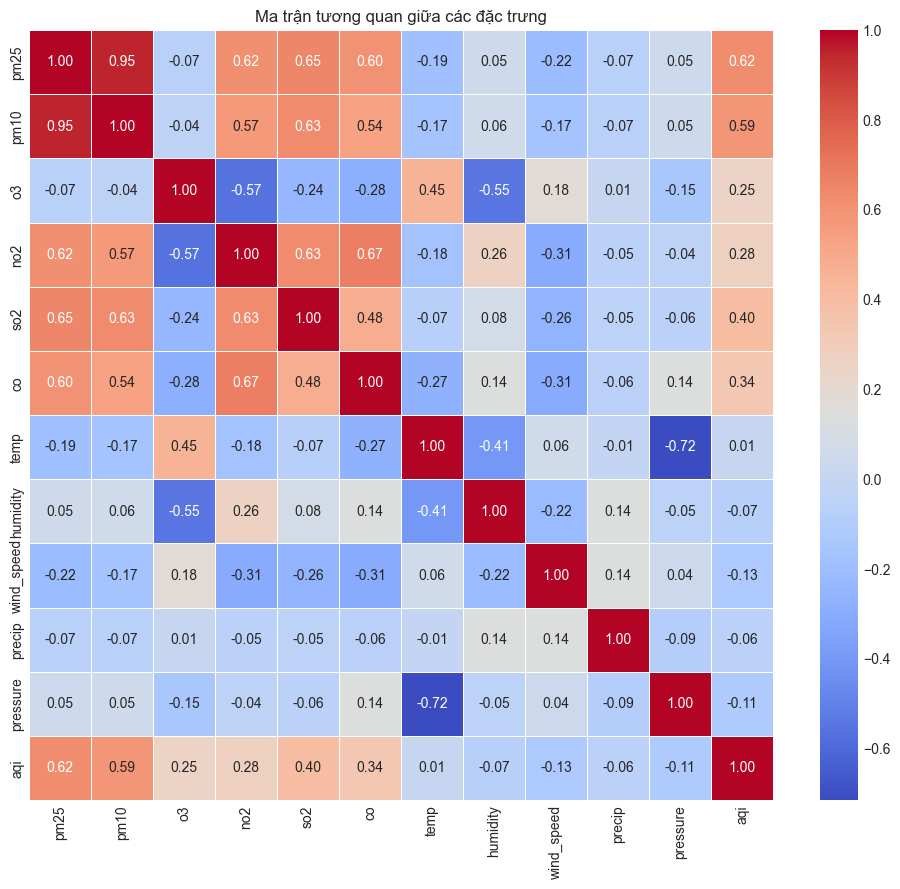
\includegraphics[width=0.72\linewidth]{eda_correlation_heatmap.png}
\caption{Ma trận tương quan Pearson giữa các biến đầu vào.}
\label{fig:eda-correlation}
\end{figure}

Tự tương quan cao ở lag ngắn cho thấy persistence là baseline mạnh: giá trị gần hiện tại thường là chỉ báo tốt cho vài giờ đầu. Tuy nhiên, tự tương quan giảm khi horizon tăng và không giải thích được hoàn toàn các cú tăng đột ngột. Chu kỳ 24 giờ gợi ý seasonal component của SARIMAX, trong khi lag 24, 48, 72 và 168 giờ cung cấp cho XGBoost thông tin cùng giờ ở các ngày trước. Với LSTM, cửa sổ 72 giờ cân bằng giữa ngữ cảnh ba ngày và chi phí huấn luyện.

EDA cũng cho thấy mất cân bằng theo miền giá trị. Phần lớn mẫu nằm ở vùng trung bình, còn Very Unhealthy và Hazardous rất hiếm. Đây là lý do một model có RMSE tổng thể tốt vẫn có thể có recall thấp ở class cực đoan. Nhóm vì vậy không dùng confusion matrix để thay thế metric hồi quy; nó chỉ bổ sung góc nhìn về lỗi có ý nghĩa sức khỏe.

\begin{figure}[H]
\centering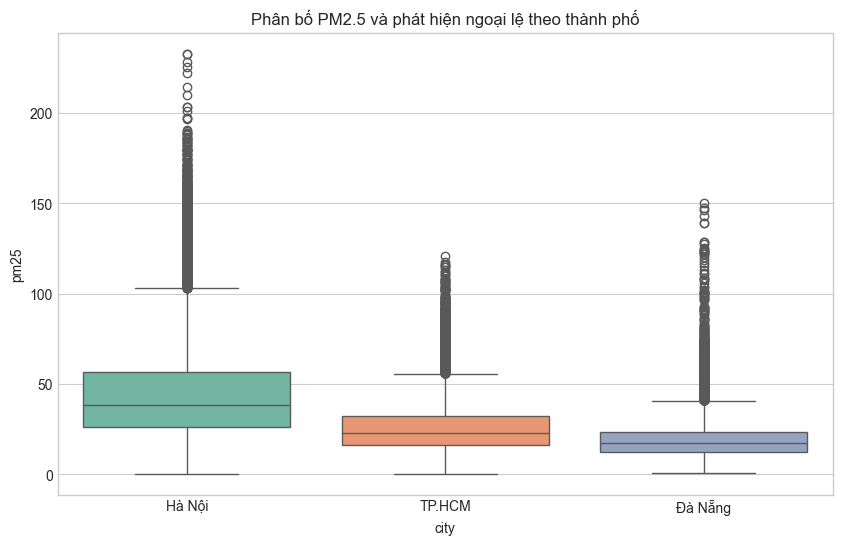
\includegraphics[width=0.84\linewidth]{eda_pm25_outliers.png}
\caption{Các điểm PM2.5 cực trị theo thành phố được phát hiện trong EDA.}
\label{fig:eda-outliers}
\end{figure}

\begin{figure}[H]
\centering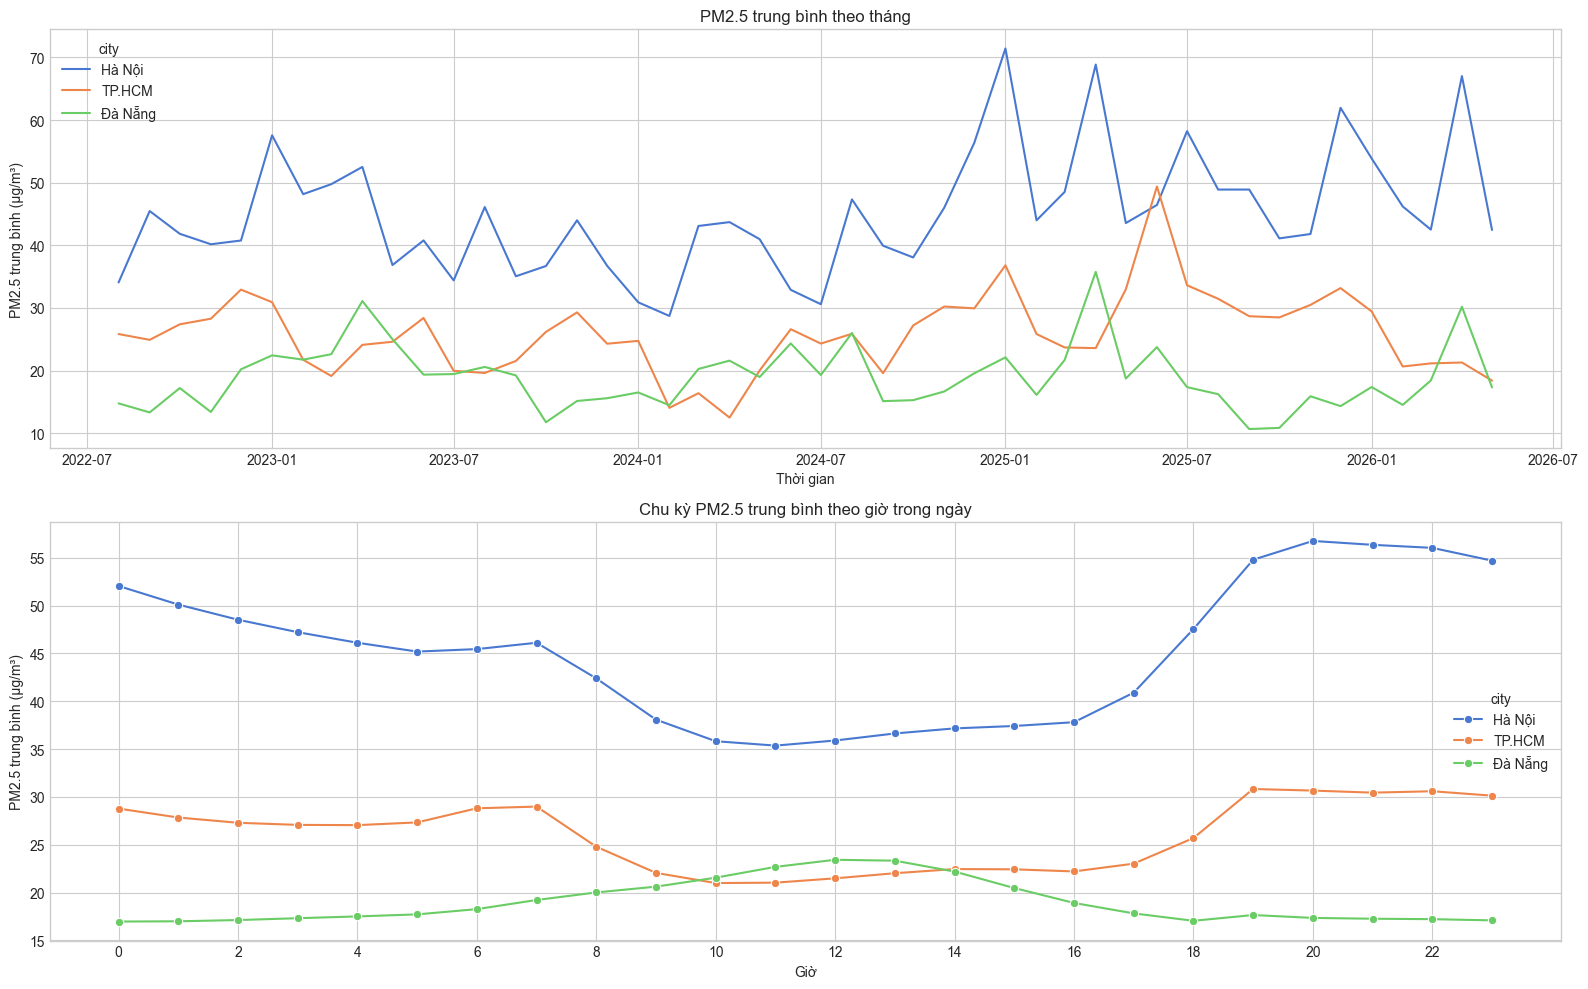
\includegraphics[width=0.92\linewidth]{eda_pm25_temporal_patterns.png}
\caption{Mẫu hình PM2.5 theo giờ và theo tháng làm cơ sở tạo đặc trưng thời gian.}
\label{fig:eda-temporal}
\end{figure}

Hình~\ref{fig:eda-outliers} và Hình~\ref{fig:eda-temporal} chỉ ra hai quyết định tiếp theo: giữ lại các đỉnh hợp lệ thay vì winsorize tự động, đồng thời tạo lag, rolling và biến chu kỳ. Các biểu đồ được sinh trực tiếp từ notebook EDA, không dùng ảnh minh họa bên ngoài dữ liệu dự án.

\subsection{Tiền xử lý và làm sạch}
Sau EDA, quy trình chuyển 13 giá trị O$_3$ âm thành thiếu, sau đó nội suy tuyến tính theo từng thành phố với giới hạn tối đa 6 giờ. PM2.5 không thiếu, dữ liệu không có khoảng thời gian phi giờ và không có bản ghi city--datetime trùng. Các đỉnh PM2.5 hợp lệ được giữ lại vì xóa chúng sẽ làm model đánh giá thấp đúng tình huống ô nhiễm nghiêm trọng cần cảnh báo.

Nội suy chỉ áp dụng cho đoạn thiếu ngắn và được thực hiện trong từng thành phố để không trộn hai chế độ khí hậu. Giới hạn 6 giờ ngăn việc dựng một chuỗi dài bằng đường thẳng khi dữ liệu nguồn mất liên tục. Với biến không thể khôi phục an toàn, hàng tương ứng sẽ không được dùng để tạo origin hợp lệ. Việc không winsorize PM2.5 là chủ đích: các đỉnh hiếm có thể làm huấn luyện khó hơn, nhưng chúng là phần có giá trị cảnh báo cao nhất. Thay vì xóa đỉnh, nhóm đánh giá riêng residual, class cực đoan và sai số theo thành phố.

Các biến số được kiểm tra kiểu dữ liệu và đơn vị trước khi tạo đặc trưng. Mã hóa mùa và thành phố được thực hiện sau khi chia theo thời gian; scaler của LSTM chỉ fit trên Train. XGBoost không cần chuẩn hóa theo thang đo, còn LSTM cần chuẩn hóa để gradient giữa các feature có độ lớn khác nhau không bị chi phối bởi một vài biến.

\subsubsection{Sáu class PM2.5 phục vụ chẩn đoán}
Đồ án là hồi quy, không huấn luyện nhãn lớp. Sau dự đoán, sáu class này do nhóm tự quy ước theo Bảng~\ref{tab:class} để lập confusion matrix và xem model bỏ lỡ vùng cực đoan nào. Các dải này không phải AQI chính thức và không được dùng làm target hay loss.

Việc tự quy ước phải được nêu rõ để tránh hai nhầm lẫn. Một là tên class chỉ giúp đọc ma trận lỗi, không khẳng định đây là hệ AQI của cơ quan quản lý. Hai là một dự đoán sai class có thể chỉ lệch rất ít nếu nằm sát ngưỡng, trong khi hai giá trị cùng class vẫn có thể cách nhau nhiều \unitpm. Vì vậy, kết luận chính luôn dựa trên RMSE, MAE, R$^2$ và residual liên tục; class chỉ dùng để phát hiện model có bỏ lỡ vùng hiếm hay không.

\begin{table}[H]
\centering\small
\caption{Các dải PM2.5 do nhóm quy ước cho phân tích lỗi}
\label{tab:class}
\begin{tabular}{lll}
\toprule
Nhãn & Khoảng PM2.5 (\unitpm) & Vai trò\\
\midrule
Good & $x\leq9.0$ & Chẩn đoán hậu xử lý\\
Moderate & $9.0<x\leq35.4$ & Chẩn đoán hậu xử lý\\
USG & $35.4<x\leq55.4$ & Nhạy cảm\\
Unhealthy & $55.4<x\leq125.4$ & Ô nhiễm cao\\
Very Unhealthy & $125.4<x\leq225.4$ & Cực đoan hiếm\\
Hazardous & $x>225.4$ & Cực đoan rất hiếm\\
\bottomrule
\end{tabular}
\end{table}

\subsection{Feature Engineering}
Sau tiền xử lý, feature engineering tạo đầu vào cho model. Tổng cộng có 68 biến số trước one-hot và 75 cột sau mã hóa thành phố, mùa. Mọi feature được tính tại thời điểm $t$ hoặc từ quá khứ.

\begin{table}[H]
\centering\small
\caption{Các nhóm đặc trưng dùng cho XGBoost Direct Multi-Horizon}
\label{tab:features}
\begin{tabular}{p{3.4cm}p{2cm}p{9.1cm}}
\toprule
Nhóm & Số lượng & Ví dụ\\
\midrule
Chất ô nhiễm & 6 & PM2.5, PM10, O$_3$, NO$_2$, SO$_2$, CO tại $t$\\
Khí tượng & 7 & Nhiệt độ, ẩm, gió, mưa, áp suất, mây\\
Thời gian & 5 & Giờ, thứ, tháng, cuối tuần, ngày trong năm\\
Lịch sử PM2.5 & 35 & Lag 1--168 giờ; mean/std/min/max 6--168 giờ; cùng giờ 7 ngày\\
Biến phái sinh & 15 & Sin/cos, ventilation, humid stagnation, wind vector, tỷ lệ PM2.5/PM10\\
Phân loại & 7 one-hot & Ba thành phố và bốn mùa\\
\bottomrule
\end{tabular}
\end{table}

Feature lịch sử giúp mô hình nhận biết quán tính ngắn hạn, chu kỳ ngày và tuần. Sin/cos tránh khoảng cách giả giữa 23 giờ và 0 giờ. Chỉ số thông gió, gió vector và độ ẩm đình trệ mô tả điều kiện khuếch tán. Tỷ lệ chất ô nhiễm là tín hiệu tương tác, nhưng feature importance không được diễn giải thành quan hệ nhân quả. Cấu trúc đầy đủ được liệt kê ở Bảng~\ref{tab:features}.

Để chống leakage, rolling mean, rolling standard deviation, min và max đều kết thúc tại origin $t$; target $t+h$ không tham gia bất kỳ phép tổng hợp nào. Feature cùng giờ tuần trước sử dụng timestamp $t-168$, không dùng phép dịch trên toàn bảng trước khi nhóm theo thành phố. Các target cũng được nối bằng khóa city--timestamp, nhờ đó một khoảng thiếu không làm lệch hàng và biến $t+24$ thành một thời điểm khác. Sau one-hot, 75 cột đầu vào được cố định thứ tự và lưu cùng artifact để backend tái tạo đúng schema lúc suy luận.

\section{Chương 3: Lựa chọn và Huấn luyện Mô hình}
\subsection{Tạo 24 target và chia dữ liệu}
Mỗi origin tạo 24 target bằng phép tra đúng timestamp trong cùng thành phố, không dùng dịch chuyển hàng mù. Dữ liệu được chia theo thời gian: Train 70\%, Validation 15\% và Test 15\%. Mốc \texttt{forecast\_end} cùng purge gap 24 giờ bảo đảm các cửa sổ target ở hai tập liền kề không giao nhau.

\begin{table}[H]
\centering\small
\caption{Temporal split của bài toán đa chân trời}
\label{tab:split}
\begin{tabular}{lrrll}
\toprule
Tập & Origin & Tỷ lệ & Source start & Source end\\
\midrule
Train & 68.829 & 70\% & 12/08/2022 07:00 & 25/03/2025 05:00\\
Validation & 14.679 & 15\% & 26/03/2025 06:00 & 16/10/2025 02:00\\
Test & 14.679 & 15\% & 17/10/2025 03:00 & 08/05/2026 23:00\\
\bottomrule
\end{tabular}
\end{table}

Bảng~\ref{tab:split} dùng tỷ lệ 70/15/15 nhưng không xáo trộn. Train đủ dài để bao phủ nhiều mùa; Validation phục vụ early stopping, tuning và lựa chọn model; Test là giai đoạn mới nhất, chỉ mở sau khi model thắng đã được xác định. Purge gap 24 giờ loại trường hợp target cuối của tập trước rơi vào thời gian nguồn của tập sau. Sau khi tạo đủ target, số origin hợp lệ giảm ở cuối mỗi chuỗi như Hình~\ref{fig:target-coverage}; đây là mất mát tất yếu vì các timestamp tương lai chưa tồn tại, không phải dữ liệu thiếu được nội suy.

\begin{figure}[H]
\centering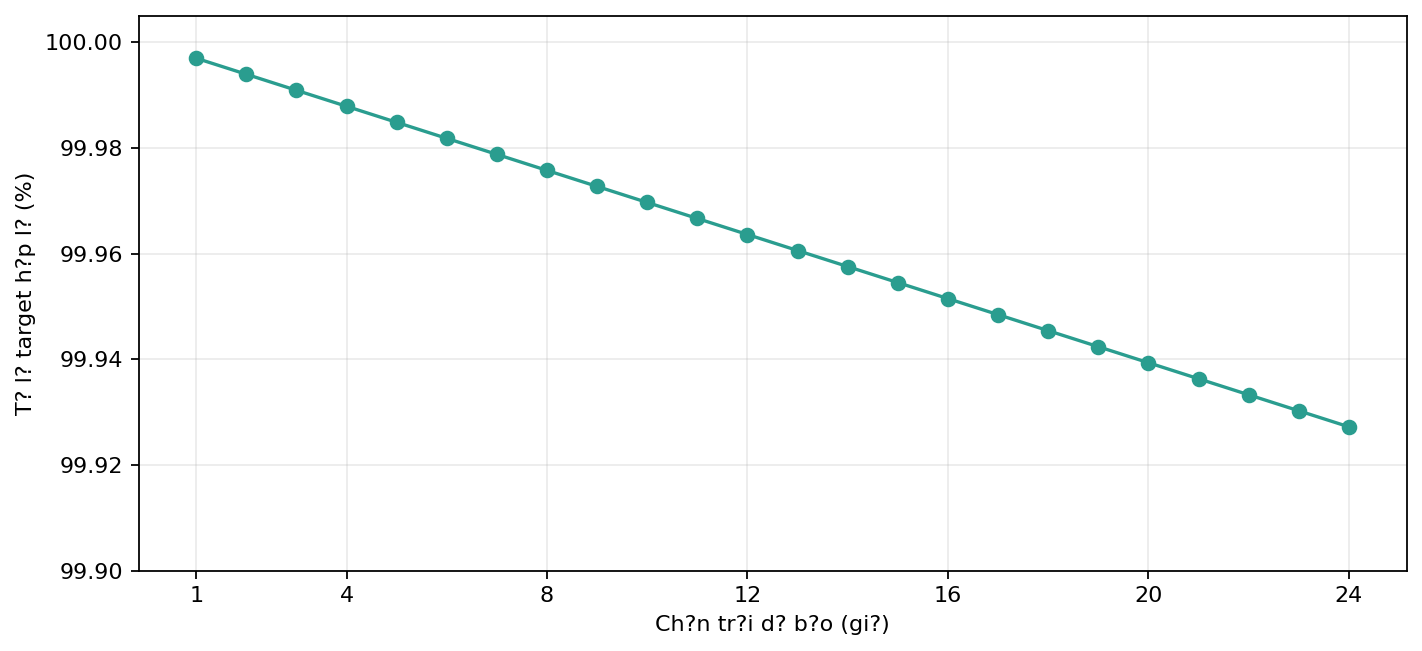
\includegraphics[width=0.78\linewidth]{target_coverage_by_horizon.png}
\caption{Tỷ lệ target hợp lệ từ $t+1$ đến $t+24$; các hàng cuối chuỗi thiếu tương lai bị loại.}
\label{fig:target-coverage}
\end{figure}

\subsection{SARIMAX đa bước}
Baseline là $\mathrm{SARIMAX}(1,0,0)\times(1,0,0)_{24}$~\cite{sarimax}, fit riêng cho từng thành phố bằng maximum likelihood và L-BFGS, tối đa 200 vòng. Dự báo 24 bước được tạo đệ quy từ hệ số AR(1), seasonal AR(24) và lịch sử PM2.5. Cả ba fit hội tụ. Ưu điểm là diễn giải được cấu trúc tự hồi quy; hạn chế là tuyến tính và sai số đệ quy tích lũy.

SARIMAX được chọn làm baseline có cấu trúc thay vì persistence đơn giản vì EDA cho thấy đồng thời quán tính ngắn hạn và chu kỳ ngày. Bậc thấp giữ số tham số nhỏ, giảm thời gian fit trên hơn hai năm dữ liệu mỗi thành phố và hạn chế bất ổn tối ưu. Mô hình không nhận toàn bộ 75 feature, nên kết quả của nó trả lời câu hỏi: chỉ với lịch sử PM2.5 và seasonality 24 giờ, mức hiệu năng có thể đạt đến đâu? Dự báo đệ quy dùng dự đoán ở bước trước làm đầu vào cho bước sau, vì vậy lỗi có khả năng tích lũy ở horizon dài.

\subsection{XGBoost Direct Multi-Horizon}
XGBoost~\cite{xgb} dùng 24 regressor độc lập, mỗi model học một target $t+h$. Cấu hình chung: 800 cây tối đa, learning rate 0,04, depth 3, min child weight 8, subsample và column sample 0,85, L1 0,05, L2 3,0, objective squared error, histogram tree và early stopping 45 vòng. Direct strategy tránh truyền lỗi từ bước trước sang bước sau nhưng tăng chi phí huấn luyện và lưu 24 model.

Gradient boosting phù hợp với bảng feature gồm lag, rolling, biến khí tượng và tương tác phi tuyến. Mỗi cây mới xấp xỉ phần residual mà ensemble hiện tại chưa giải thích. Learning rate thấp kết hợp tối đa 800 cây cho phép cập nhật nhỏ; depth 3 và min child weight 8 ngăn cây chia quá sâu trên các trường hợp hiếm. Subsample và column sample 0,85 tạo ngẫu nhiên ở cả hàng và cột, còn regularization L1/L2 phạt độ phức tạp của leaf. Early stopping theo Validation RMSE chọn số boosting round riêng cho từng horizon thay vì mặc định dùng đủ 800 cây.

Việc dùng 24 model direct có hai hệ quả. Mặt tích cực là model $t+24$ không phụ thuộc dự đoán $t+23$, nên lỗi không truyền theo chuỗi như SARIMAX recursive. Mặt hạn chế là 24 đầu ra không bị ràng buộc phải tạo một đường dự báo trơn và chi phí artifact tăng tuyến tính theo số horizon. Web vì vậy tải một bundle chứa schema chung và danh sách regressor, rồi chọn đúng model theo horizon người dùng yêu cầu.

\subsection{LSTM Sequence-to-Vector}
LSTM~\cite{lstm} nhận chuỗi 72 giờ, 16 feature và xuất đồng thời 24 giá trị. Kiến trúc gồm LSTM 96, LSTM 48, Dense 64 ReLU có L2, Dropout 0,20 và Dense 24 tuyến tính; tổng cộng 75.928 tham số. Feature và target chỉ được chuẩn hóa bằng scaler fit trên Train. Loss là MSE, optimizer Adam với learning rate $10^{-3}$, batch 256, tối đa 60 epoch, Early Stopping patience 10 và ReduceLROnPlateau patience 5.

Hai tầng LSTM tách việc mã hóa động lực cục bộ và cô đọng chuỗi thành vector trạng thái. Tầng đầu trả toàn bộ sequence cho tầng thứ hai; tầng thứ hai trả vector cuối, Dense 64 học kết hợp phi tuyến trước đầu ra 24 chiều. Hàm kích hoạt cổng sigmoid và trạng thái tanh là cấu trúc chuẩn của LSTM, Dense giữa dùng ReLU, còn Dense cuối dùng linear vì target là số thực không âm nhưng model cần gradient không bão hòa. Giá trị âm nếu có được chặn ở bước phục vụ, không dùng activation ReLU ở output để tránh làm sai động lực tối ưu gần 0.

MSE là loss huấn luyện vì phạt mạnh sai số lớn ở các đỉnh, trong khi MAE và RMSE được theo dõi để hiểu cả sai số điển hình lẫn sai số nhạy với cực trị. Adam điều chỉnh learning rate theo tham số; ReduceLROnPlateau giảm bước học khi Validation loss không cải thiện. Dropout, L2 và Early Stopping là ba tầng kiểm soát overfitting. Hình~\ref{fig:lstm-architecture} mô tả kích thước tensor và số tham số, còn Hình~\ref{fig:lstm-curves} cho thấy quá trình học thực tế.

\begin{figure}[H]
\centering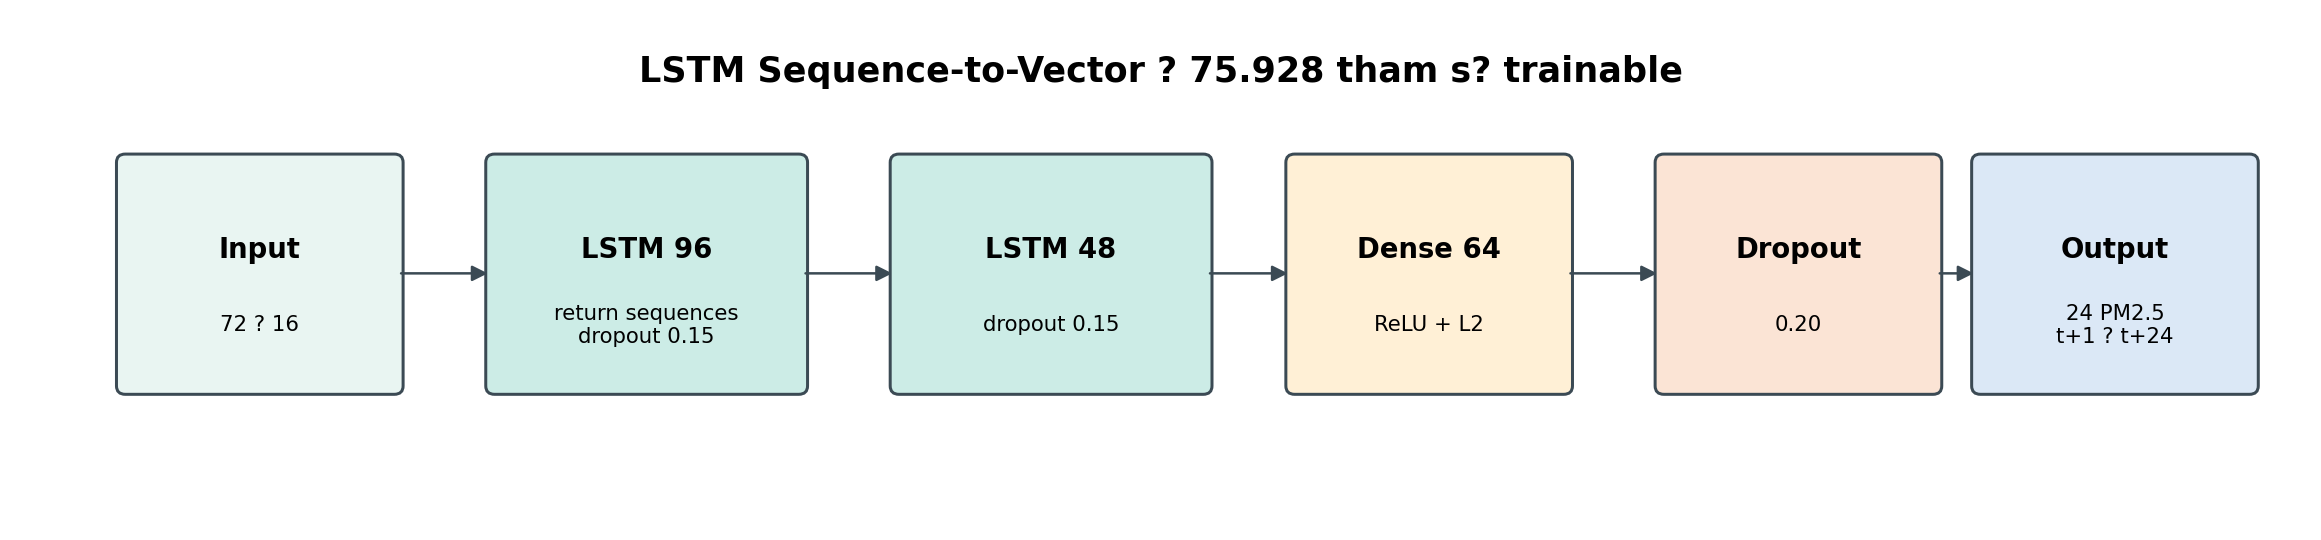
\includegraphics[width=0.96\linewidth]{lstm_multihorizon_architecture.png}
\caption{Kiến trúc LSTM Sequence-to-Vector đúng theo notebook trong thư mục \texttt{model}.}
\label{fig:lstm-architecture}
\end{figure}

\begin{figure}[H]
\centering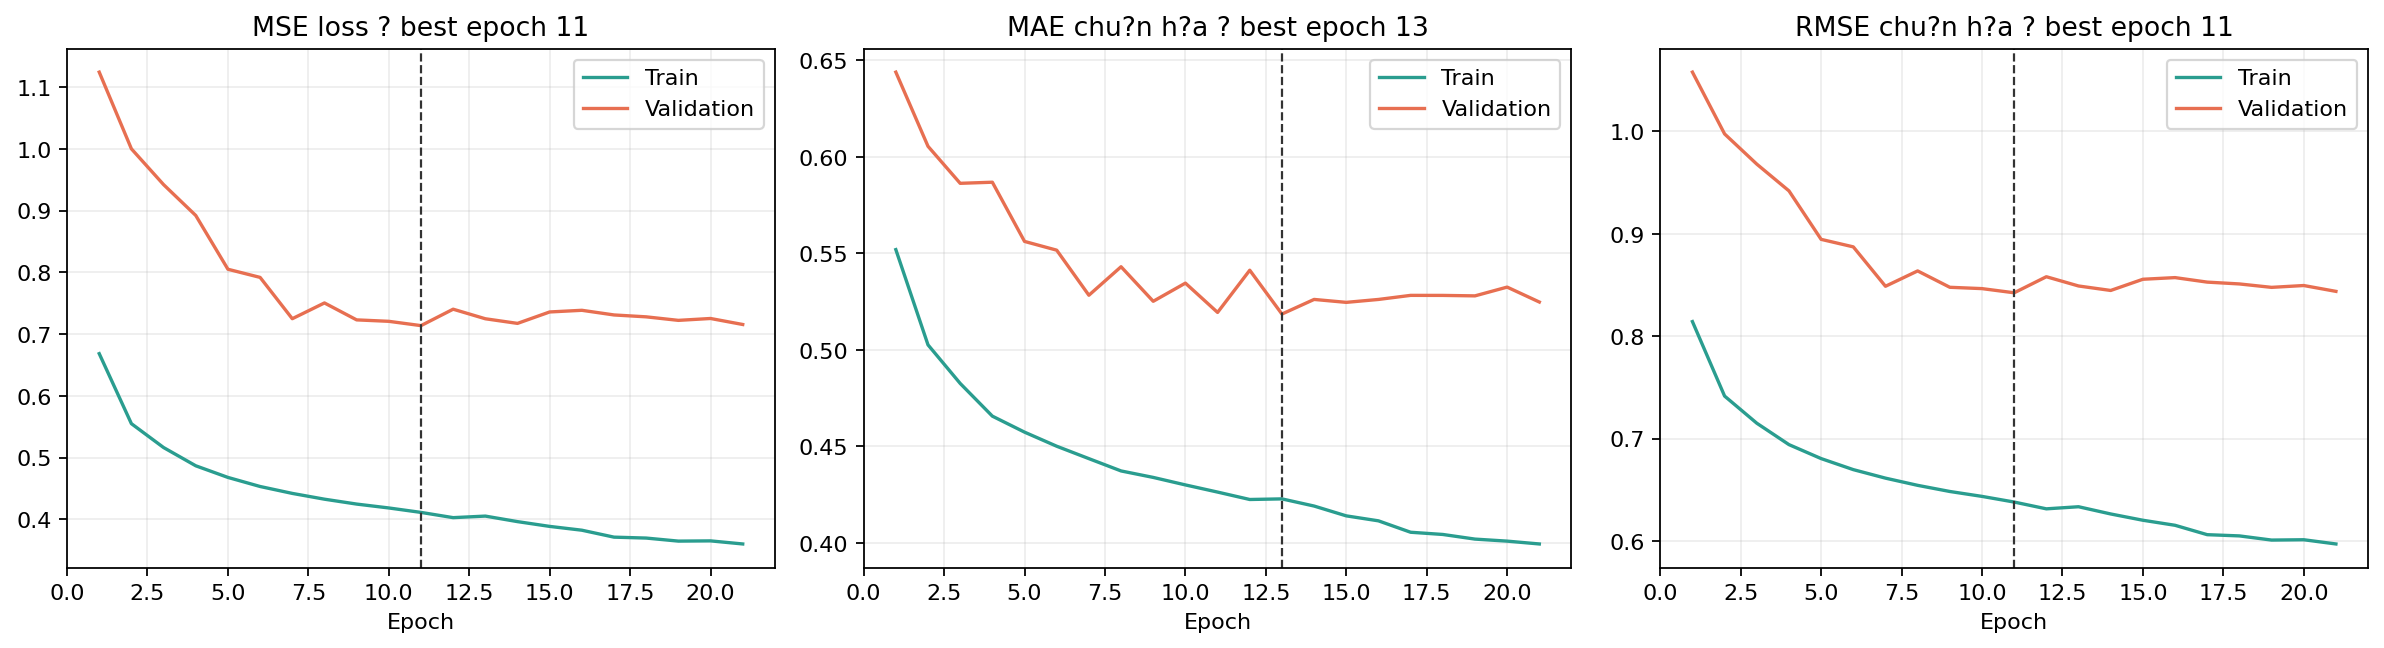
\includegraphics[width=0.98\linewidth]{lstm_multihorizon_training_curves.png}
\caption{Learning curves MSE, MAE và RMSE chuẩn hóa của LSTM trên Train và Validation.}
\label{fig:lstm-curves}
\end{figure}

Validation loss LSTM tốt nhất ở epoch 11. Sau điểm này Train tiếp tục cải thiện nhưng Validation không giảm bền vững, cho thấy overfitting; Early Stopping khôi phục trọng số tốt nhất. XGBoost dùng Validation RMSE tại từng horizon để early stop. SARIMAX không huấn luyện theo epoch nên trạng thái hội tụ và AIC thay cho learning curve.

\subsection{Hàm mục tiêu, metric và cấu hình huấn luyện}
Với $N$ mẫu, sai số ở một horizon được đánh giá bởi
\begin{align}
\mathrm{MSE} &= \frac{1}{N}\sum_{i=1}^{N}(y_i-\hat y_i)^2, &
\mathrm{RMSE} &= \sqrt{\mathrm{MSE}},\\
\mathrm{MAE} &= \frac{1}{N}\sum_{i=1}^{N}|y_i-\hat y_i|, &
R^2 &= 1-\frac{\sum_i(y_i-\hat y_i)^2}{\sum_i(y_i-\bar y)^2}.
\end{align}
RMSE cùng đơn vị với PM2.5 và nhạy với đỉnh; MAE dễ diễn giải như sai lệch tuyệt đối điển hình; $R^2$ đo phần phương sai được giải thích so với dự báo trung bình. Không dùng Accuracy làm metric chính vì đây là hồi quy. Accuracy, Precision, Recall và F1 chỉ xuất hiện sau khi ánh xạ dự đoán liên tục sang sáu dải do nhóm quy ước.

\begin{table}[H]
\centering\small
\caption{Cấu hình huấn luyện chính của ba mô hình}
\label{tab:training}
\begin{tabular}{p{2.5cm}p{4.0cm}p{4.0cm}p{4.1cm}}
\toprule
Thành phần & SARIMAX & XGBoost & LSTM\\
\midrule
Đầu vào & PM2.5 theo thành phố & 75 feature dạng bảng & 72 giờ $\times$ 16 feature\\
Đầu ra & 24 bước đệ quy & 24 regressor direct & Vector 24 giá trị\\
Mục tiêu & Maximum likelihood & Squared error & MSE\\
Tối ưu & L-BFGS, 200 vòng & Boosting, lr 0,04 & Adam, lr $10^{-3}$\\
Regularization & Bậc mô hình thấp & Depth, sampling, L1/L2 & Dropout, L2, Early Stop\\
Tiêu chí dừng & Hội tụ likelihood & 45 vòng không cải thiện & Patience 10; giảm lr 5\\
\bottomrule
\end{tabular}
\end{table}

Bảng~\ref{tab:training} cho thấy ba model không được ép dùng cùng một optimizer hay loss nội bộ; sự công bằng nằm ở target, split và metric đánh giá giống nhau. Siêu tham số được chọn bằng thử nghiệm có kiểm soát trên Validation và regularization, không dùng Test để tinh chỉnh. Với XGBoost, early stopping còn chọn số cây riêng cho từng horizon. Với LSTM, kiến trúc và batch được giữ cố định trong một lần huấn luyện để learning curve có thể so sánh trực tiếp.

\subsection{Giao thức lựa chọn model}
Thay vì dùng một Validation RMSE duy nhất, giai đoạn Validation được chia thành năm khối thời gian liên tiếp. Trên mỗi khối, RMSE được tính riêng cho 24 horizon rồi lấy trung bình. Model được chọn theo RMSE trung bình qua năm khối; độ lệch chuẩn, worst-fold RMSE và MAE là tiêu chí phụ. Đây là blocked temporal validation trên các candidate đã fit, không phải K-fold ngẫu nhiên và không tuyên bố đã refit ba model năm lần. Test bị khóa cho đến khi tên model thắng được xác định. Cách chia block giữ nguyên thứ tự thời gian và đánh giá model qua nhiều regime liên tiếp, phù hợp hơn K-fold xáo trộn cho dự báo chuỗi~\cite{tashman}.

Giao thức hiện tại là kiểm tra độ ổn định của prediction đã sinh trên Validation, không phải strict rolling-origin CV. Một rolling-origin CV đầy đủ sẽ fit lại từng model ở mỗi cutoff, tốn đáng kể thời gian cho SARIMAX và LSTM nhưng phản ánh tốt hơn quy trình tái huấn luyện thực tế. Báo cáo phân biệt rõ hai khái niệm để không diễn giải năm block như năm lần huấn luyện độc lập.

\section{Chương 4: Kết quả và Thảo luận}
\subsection{Kết quả temporal cross-validation}
\begin{table}[H]
\centering\small
\caption{Kết quả năm khối Validation; RMSE và MAE có đơn vị \unitpm}
\label{tab:cv}
\begin{tabular}{lrrrrr}
\toprule
Model & CV RMSE mean & CV RMSE std & Worst fold & CV MAE & Fold thắng\\
\midrule
XGBoost & \textbf{15,80} & 1,32 & 18,08 & \textbf{9,76} & \textbf{5/5}\\
LSTM & 16,79 & 2,16 & 20,63 & 10,50 & 0/5\\
SARIMAX & 17,69 & 1,65 & 20,25 & 10,99 & 0/5\\
\bottomrule
\end{tabular}
\end{table}

\begin{figure}[H]
\centering
\begin{subfigure}{0.49\linewidth}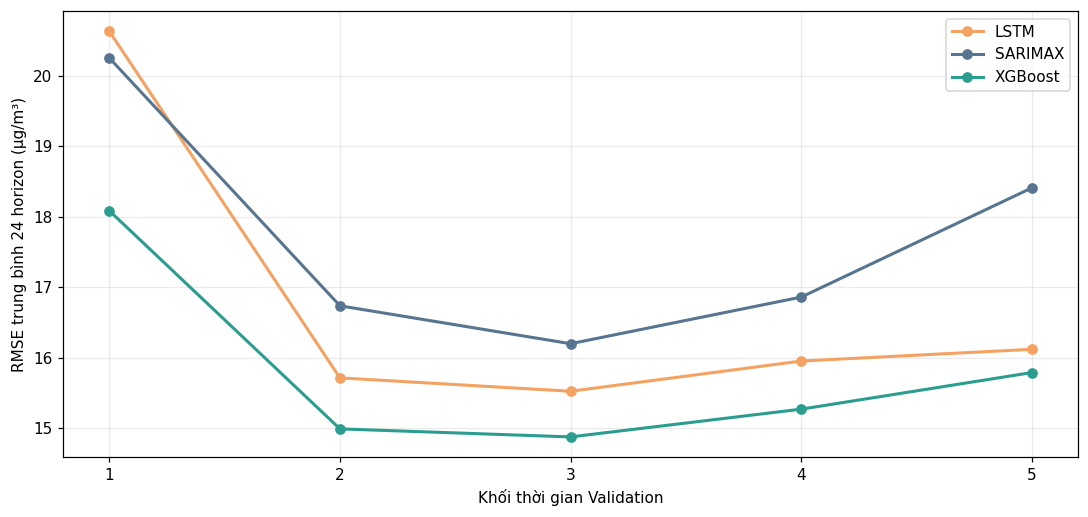
\includegraphics[width=\linewidth]{temporal_cv_fold_rmse.png}\caption{RMSE từng fold}\end{subfigure}
\begin{subfigure}{0.49\linewidth}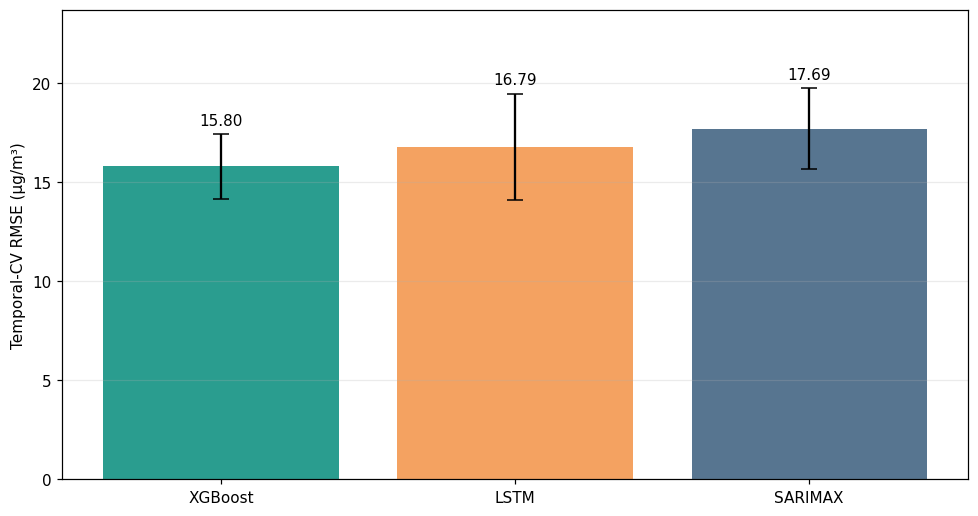
\includegraphics[width=\linewidth]{temporal_cv_model_selection.png}\caption{RMSE trung bình và CI 95\%}\end{subfigure}
\caption{Blocked temporal validation của ba candidate trên năm giai đoạn liên tiếp.}
\label{fig:cv}
\end{figure}

Theo Bảng~\ref{tab:cv} và Hình~\ref{fig:cv}, XGBoost đứng đầu ở cả năm fold, thấp hơn LSTM 0,99 \unitpm và thấp hơn SARIMAX 1,89 \unitpm theo RMSE trung bình. Độ lệch chuẩn 1,32 cũng nhỏ nhất, còn worst fold 18,08 thấp hơn hai đối thủ. Kết quả đồng thuận 5/5 block là bằng chứng mạnh hơn một Validation score duy nhất vì nó cho thấy thứ hạng không chỉ do một đoạn thời gian thuận lợi.

Tuy nhiên, khoảng tin cậy giữa XGBoost và LSTM còn chồng lấn. Năm block cũng không độc lập hoàn toàn vì cùng thuộc một chuỗi và các dự báo có horizon chồng lấn. Vì vậy, kết quả chỉ cho thấy XGBoost ổn định hơn trên dữ liệu hiện có, không chứng minh ưu thế tuyệt đối trên mọi phân phối tương lai. Khi có thêm năm dữ liệu, cần lặp lại rolling-origin evaluation và kiểm tra thứ hạng theo mùa.

\subsection{Đánh giá Test}
Sau khi khóa XGBoost, Test được mở. Bảng~\ref{tab:test} cho thấy XGBoost vẫn có RMSE và MAE thấp nhất, đồng thời R$^2$ cao nhất. Chênh lệch giữa CV và Test ở Hình~\ref{fig:cv-test} không được dùng để chọn lại model; nó chỉ kiểm tra khả năng tổng quát hóa sang giai đoạn mới nhất.

\begin{table}[H]
\centering\small
\caption{Hiệu năng Test trung bình trên 24 horizon}
\label{tab:test}
\begin{tabular}{lrrr}
\toprule
Model & RMSE (\unitpm) & MAE (\unitpm) & Global R$^2$\\
\midrule
XGBoost & \textbf{14,01} & \textbf{8,91} & \textbf{0,665}\\
LSTM & 15,26 & 9,89 & 0,619\\
SARIMAX & 16,01 & 9,85 & 0,566\\
\bottomrule
\end{tabular}
\end{table}

\begin{figure}[H]
\centering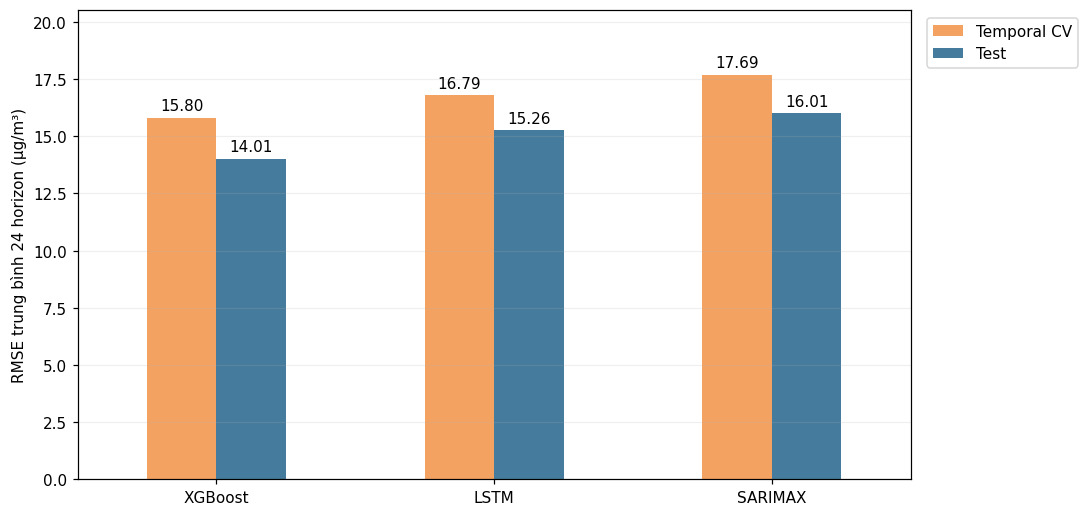
\includegraphics[width=0.75\linewidth]{cv_vs_test_model_comparison.png}
\caption{So sánh temporal-CV và Test RMSE; Test không tham gia lựa chọn model.}
\label{fig:cv-test}
\end{figure}

XGBoost cải thiện Test RMSE khoảng 8,2\% so với LSTM và 12,5\% so với SARIMAX; MAE thấp hơn khoảng 10\% so với cả hai. Global $R^2=0,665$ cho thấy model giải thích được phần lớn nhưng chưa phải toàn bộ biến thiên. Việc LSTM không thắng không mâu thuẫn với bản chất học sâu: ưu thế của mô hình phụ thuộc dữ liệu, biểu diễn, mục tiêu và mức tuning. Với khoảng 98 nghìn bản ghi, feature tabular giàu lịch sử và ba thành phố, inductive bias của boosting cây có thể phù hợp hơn một mạng 75.928 tham số.

\begin{figure}[H]
\centering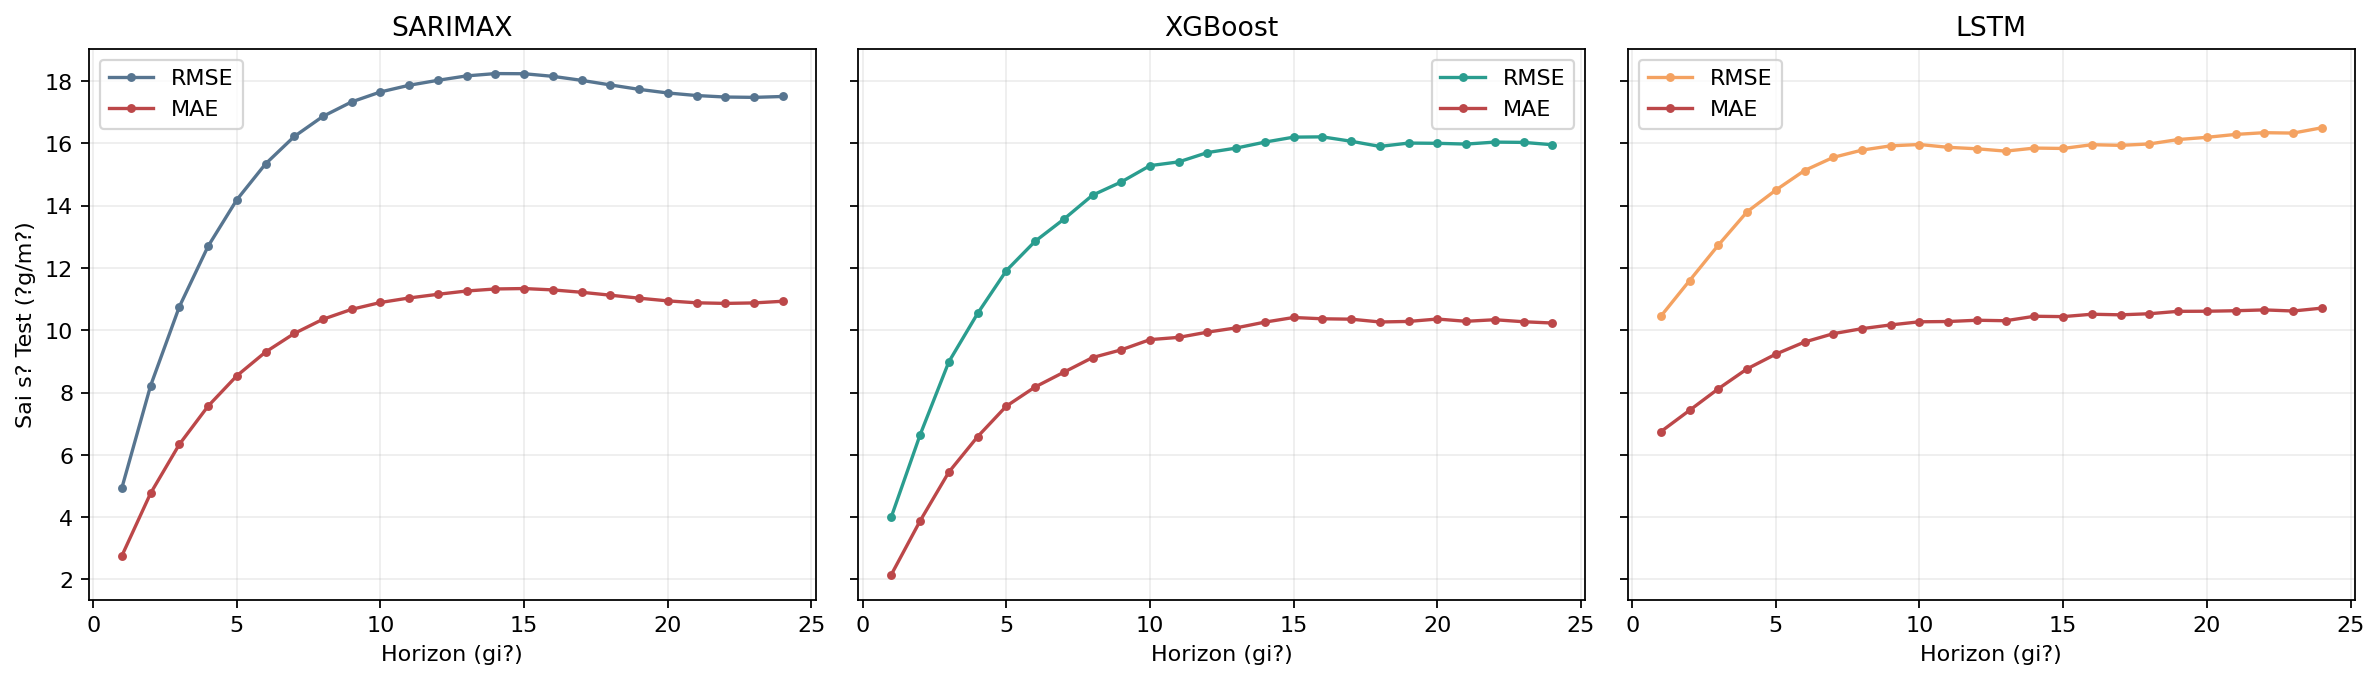
\includegraphics[width=0.98\linewidth]{three_models_error_by_horizon.png}
\caption{RMSE và MAE Test theo horizon của SARIMAX, XGBoost và LSTM.}
\label{fig:all-horizon}
\end{figure}

Hình~\ref{fig:all-horizon} cho thấy cả ba model đều khó dần khi horizon tăng, nhưng hình dạng đường sai số khác nhau. SARIMAX chịu tích lũy lỗi do chiến lược recursive. LSTM xuất đồng thời 24 bước nên đường sai số tương đối trơn, nhưng không tận dụng các feature bảng tốt bằng XGBoost. XGBoost giữ lợi thế tại phần lớn horizon, đặc biệt ở ngắn hạn, nhờ lag và rolling gần origin.

\subsection{Sai số theo horizon và thành phố}
XGBoost RMSE tăng từ 4,01 \unitpm ở $t+1$ lên 15,96 \unitpm ở $t+24$; horizon khó nhất là $t+16$ với 16,21 \unitpm. Xu hướng tăng là hợp lý vì tín hiệu tại $t$ mất dần giá trị khi khoảng dự báo dài hơn. MAE tăng chậm hơn RMSE, hàm ý một phần khoảng cách đến từ một số sai số rất lớn thay vì toàn bộ dự báo đều xấu. Hình~\ref{fig:horizon-city} đồng thời cho thấy độ khó theo horizon và theo địa lý.

\begin{figure}[H]
\centering
\begin{subfigure}{0.55\linewidth}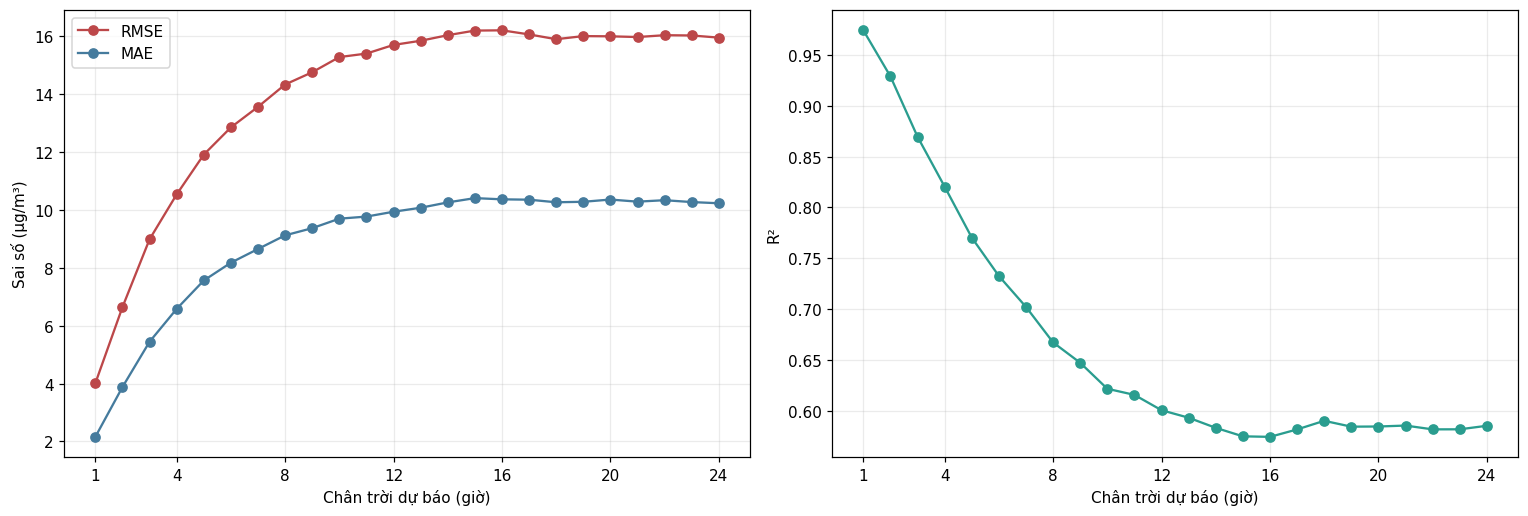
\includegraphics[width=\linewidth]{best_model_metrics_by_horizon.png}\caption{Metric theo horizon}\end{subfigure}
\begin{subfigure}{0.43\linewidth}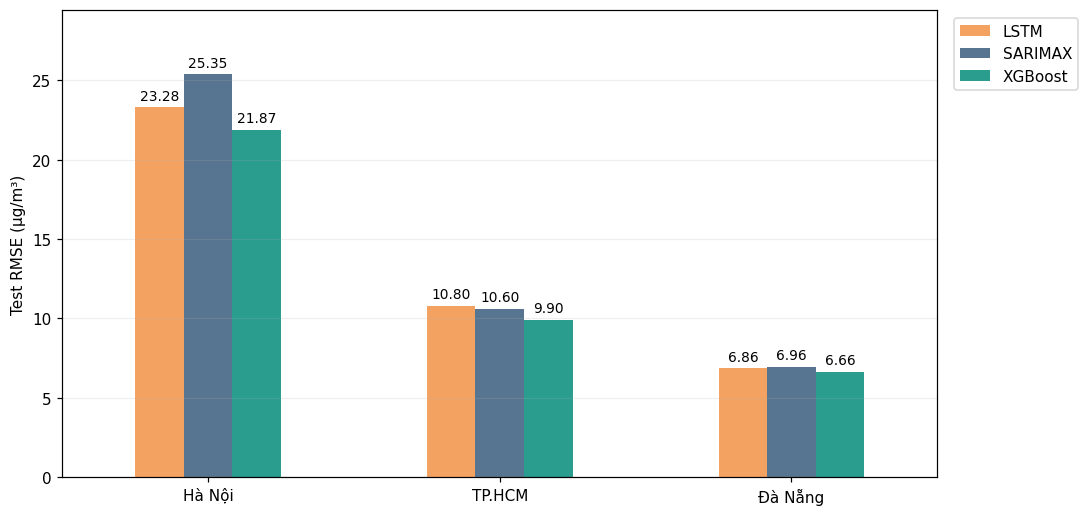
\includegraphics[width=\linewidth]{test_rmse_by_city.png}\caption{RMSE theo thành phố}\end{subfigure}
\caption{Độ khó theo thời gian và địa lý của bài toán dự báo đa chân trời.}
\label{fig:horizon-city}
\end{figure}

Hà Nội khó nhất với RMSE 21,87 \unitpm, TP.HCM 9,90 và Đà Nẵng 6,66. Hà Nội có nhiều đỉnh PM2.5 và phương sai cao hơn; một metric tổng hợp sẽ che giấu failure mode địa lý này. Sai số không đồng đều còn cảnh báo rằng một khoảng bất định toàn cục sẽ quá hẹp cho Hà Nội nhưng quá rộng cho hai thành phố còn lại. Vì thế bước conformal được hiệu chỉnh riêng theo city--horizon.

\subsection{Overfitting và feature importance}
Ở bốn horizon đại diện, khoảng cách Train--Validation RMSE tại best round trung bình 4,30 \unitpm. Khoảng cách tăng ở horizon dài cho thấy cây vẫn fit Train sát hơn Validation. Early stopping, depth 3, min child weight 8, subsampling và L1/L2 làm giảm nhưng không loại bỏ overfitting. Hình~\ref{fig:xgb-learning} cho thấy Validation RMSE giảm nhanh ở giai đoạn đầu rồi chững, trong khi Train tiếp tục giảm; best round phải lấy tại cực tiểu Validation, không phải vòng cuối.

LSTM biểu hiện mẫu tương tự nhưng theo epoch: Validation loss tốt nhất ở epoch 11 rồi dao động/tăng nhẹ trong khi Train loss tiếp tục giảm. Early Stopping đã khôi phục checkpoint tốt nhất nên tránh dùng trạng thái epoch 60. SARIMAX không có learning curve Train--Validation theo epoch; thay vào đó kiểm tra cờ hội tụ, AIC và sai số out-of-sample. Không model nào có dấu hiệu underfitting thuần túy vì Train error đều thấp hơn rõ Validation/Test, nhưng XGBoost và LSTM vẫn còn generalization gap.

\begin{figure}[H]
\centering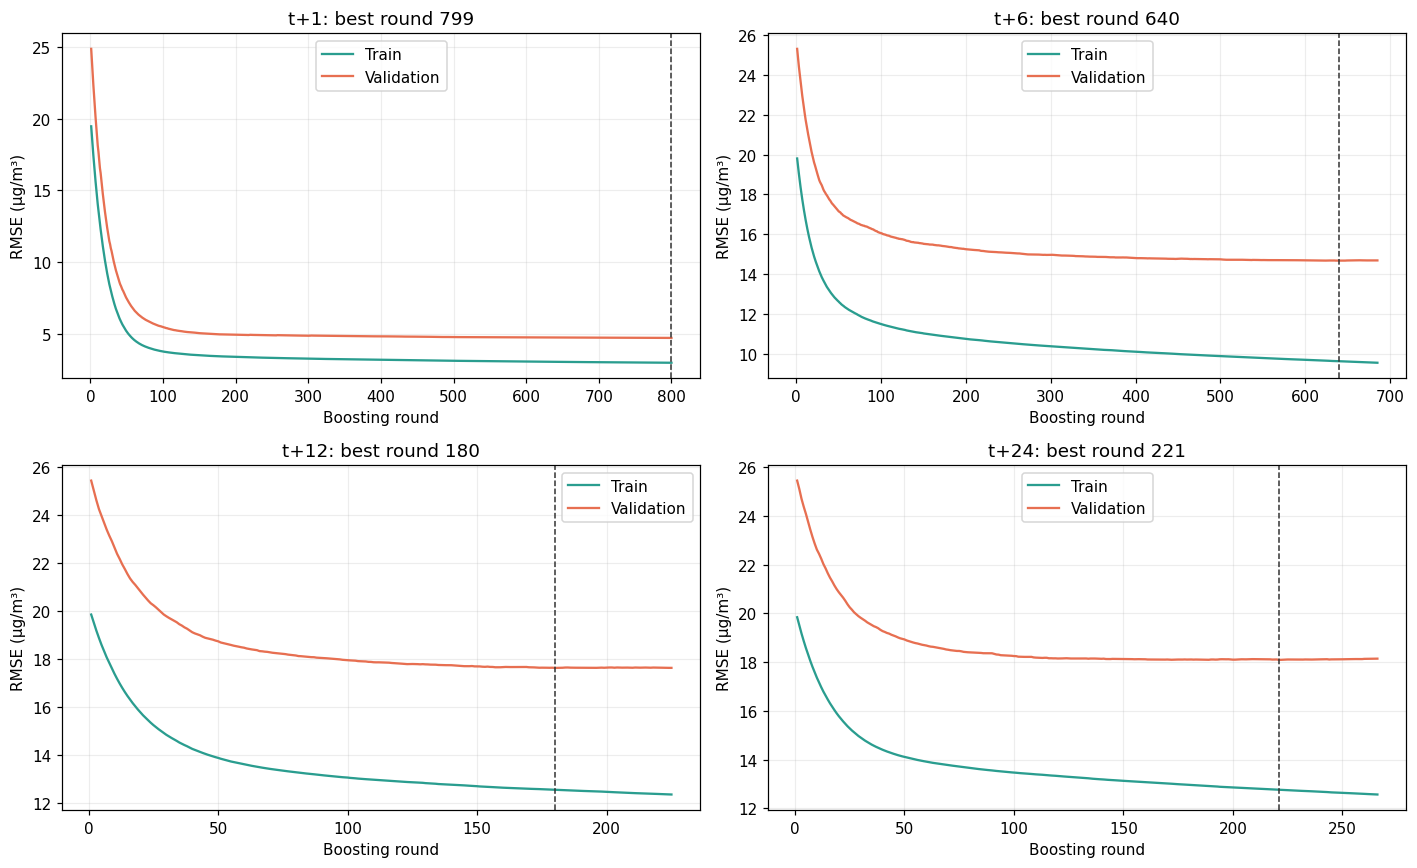
\includegraphics[width=0.96\linewidth]{best_model_learning_curves.png}
\caption{Learning curves XGBoost tại $t+1$, $t+6$, $t+12$ và $t+24$; đường đứt là best round.}
\label{fig:xgb-learning}
\end{figure}

\begin{figure}[H]
\centering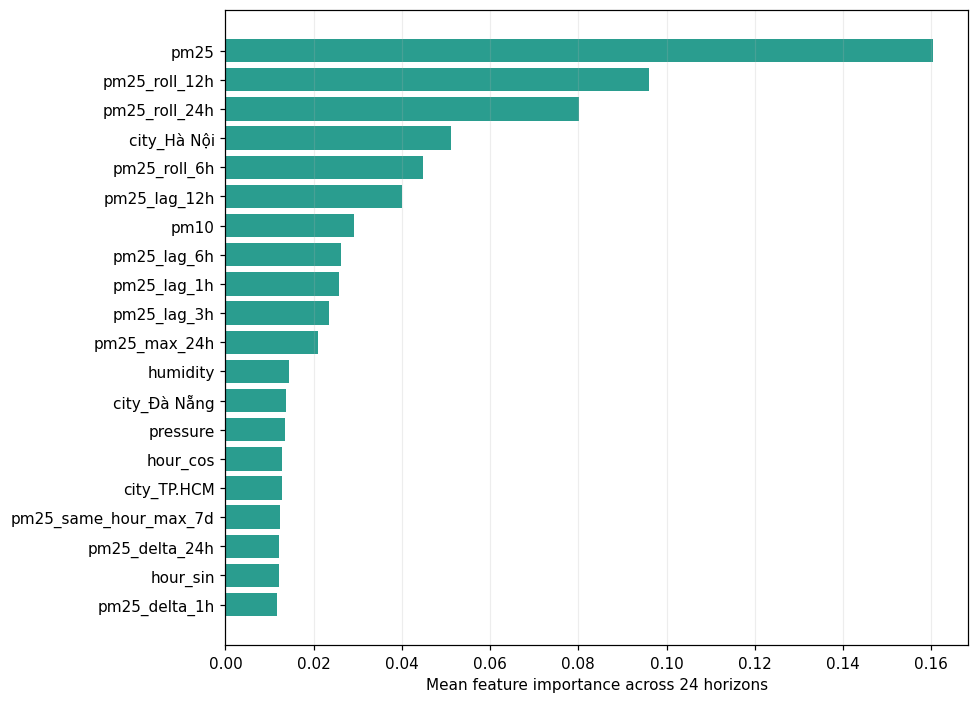
\includegraphics[width=0.72\linewidth]{best_model_feature_importance.png}
\caption{Hai mươi feature có importance trung bình cao nhất qua 24 XGBoost.}
\label{fig:importance}
\end{figure}

Hình~\ref{fig:importance} cho thấy PM2.5 hiện tại, rolling 12 giờ, rolling 24 giờ, lag và PM10 chiếm vai trò lớn. Biến one-hot Hà Nội phản ánh khác biệt regime địa lý. Importance chỉ mô tả mức model sử dụng biến, không chứng minh tác động nhân quả. Các feature tương quan có thể chia sẻ importance hoặc thay thế nhau; muốn diễn giải ổn định hơn cần permutation importance theo block thời gian hoặc SHAP có kiểm tra tương quan.

\subsection{Khoảng dự báo conformal}
Absolute residual trên Validation được dùng để hiệu chỉnh bán kính riêng theo thành phố và horizon theo nguyên lý conformal prediction~\cite{conformal}. Với dự báo điểm $\hat y$, khoảng đối xứng là $[\hat y-q_{0.9},\hat y+q_{0.9}]$, trong đó $q_{0.9}$ là quantile hữu hạn mẫu của $|y-\hat y|$ trên calibration tương ứng. Trên Test, coverage tổng hợp đạt 92,4\%, gần và hơi bảo thủ so với mục tiêu 90\%. Coverage theo thành phố là 89,1\% ở Hà Nội, 94,9\% ở TP.HCM và 93,2\% ở Đà Nẵng. Khoảng rộng hơn tại Hà Nội vì sai số lớn hơn. Hình~\ref{fig:conformal} trình bày coverage và độ rộng theo từng horizon.

\begin{figure}[H]
\centering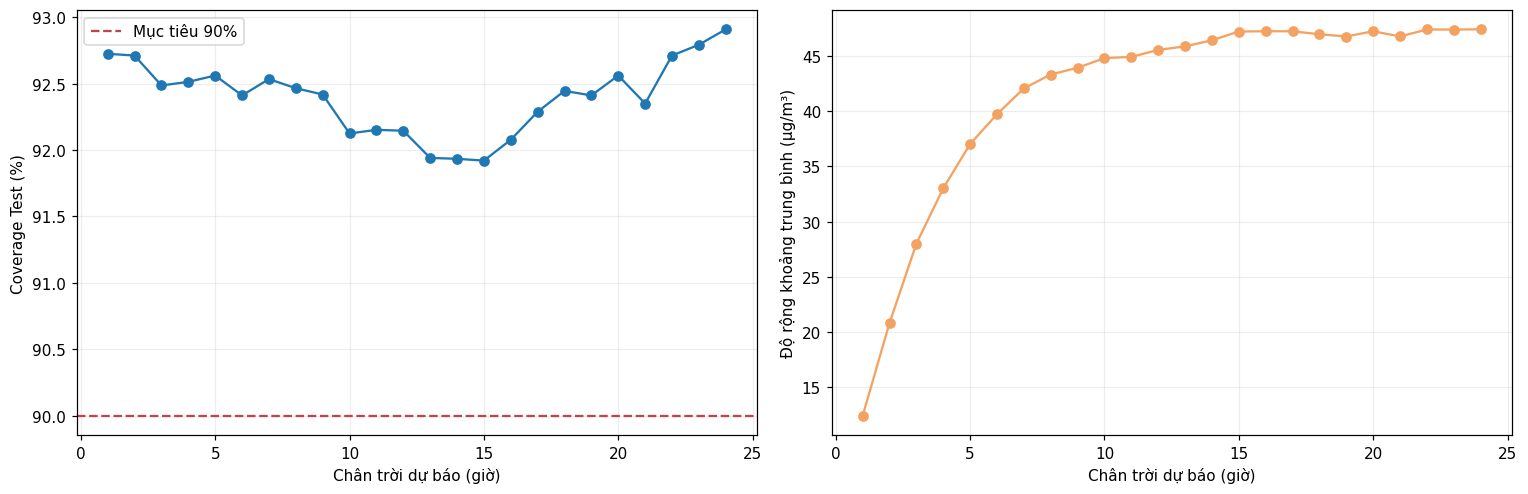
\includegraphics[width=0.86\linewidth]{best_model_conformal_coverage.png}
\caption{Coverage và độ rộng khoảng conformal 90\% theo horizon trên Test.}
\label{fig:conformal}
\end{figure}

Conformal prediction mô tả bất định thực nghiệm dưới giả định calibration và dữ liệu tương lai có tính trao đổi gần đúng. Dữ liệu ô nhiễm có drift và phụ thuộc thời gian, nên coverage cần được giám sát và hiệu chỉnh lại định kỳ; khoảng dự báo không phải bảo đảm cho từng thời điểm.

\subsection{Dự báo trực quan trên phần cuối Test}
Để kiểm tra model có bám được diễn biến chuỗi thay vì chỉ nhìn metric tổng hợp, Hình~\ref{fig:test-forecast} lấy riêng lát cắt $t+24$ của XGBoost đa chân trời trên 240 giờ mục tiêu cuối của Test. Chọn một horizon cố định bảo đảm mỗi target time chỉ có một dự báo, nhờ đó đường thời gian có thể đọc trực tiếp và so sánh công bằng với model $t+24$ cũ. Khoảng conformal trong hình vẫn được hiệu chỉnh hoàn toàn bằng Validation.

\begin{figure}[H]
\centering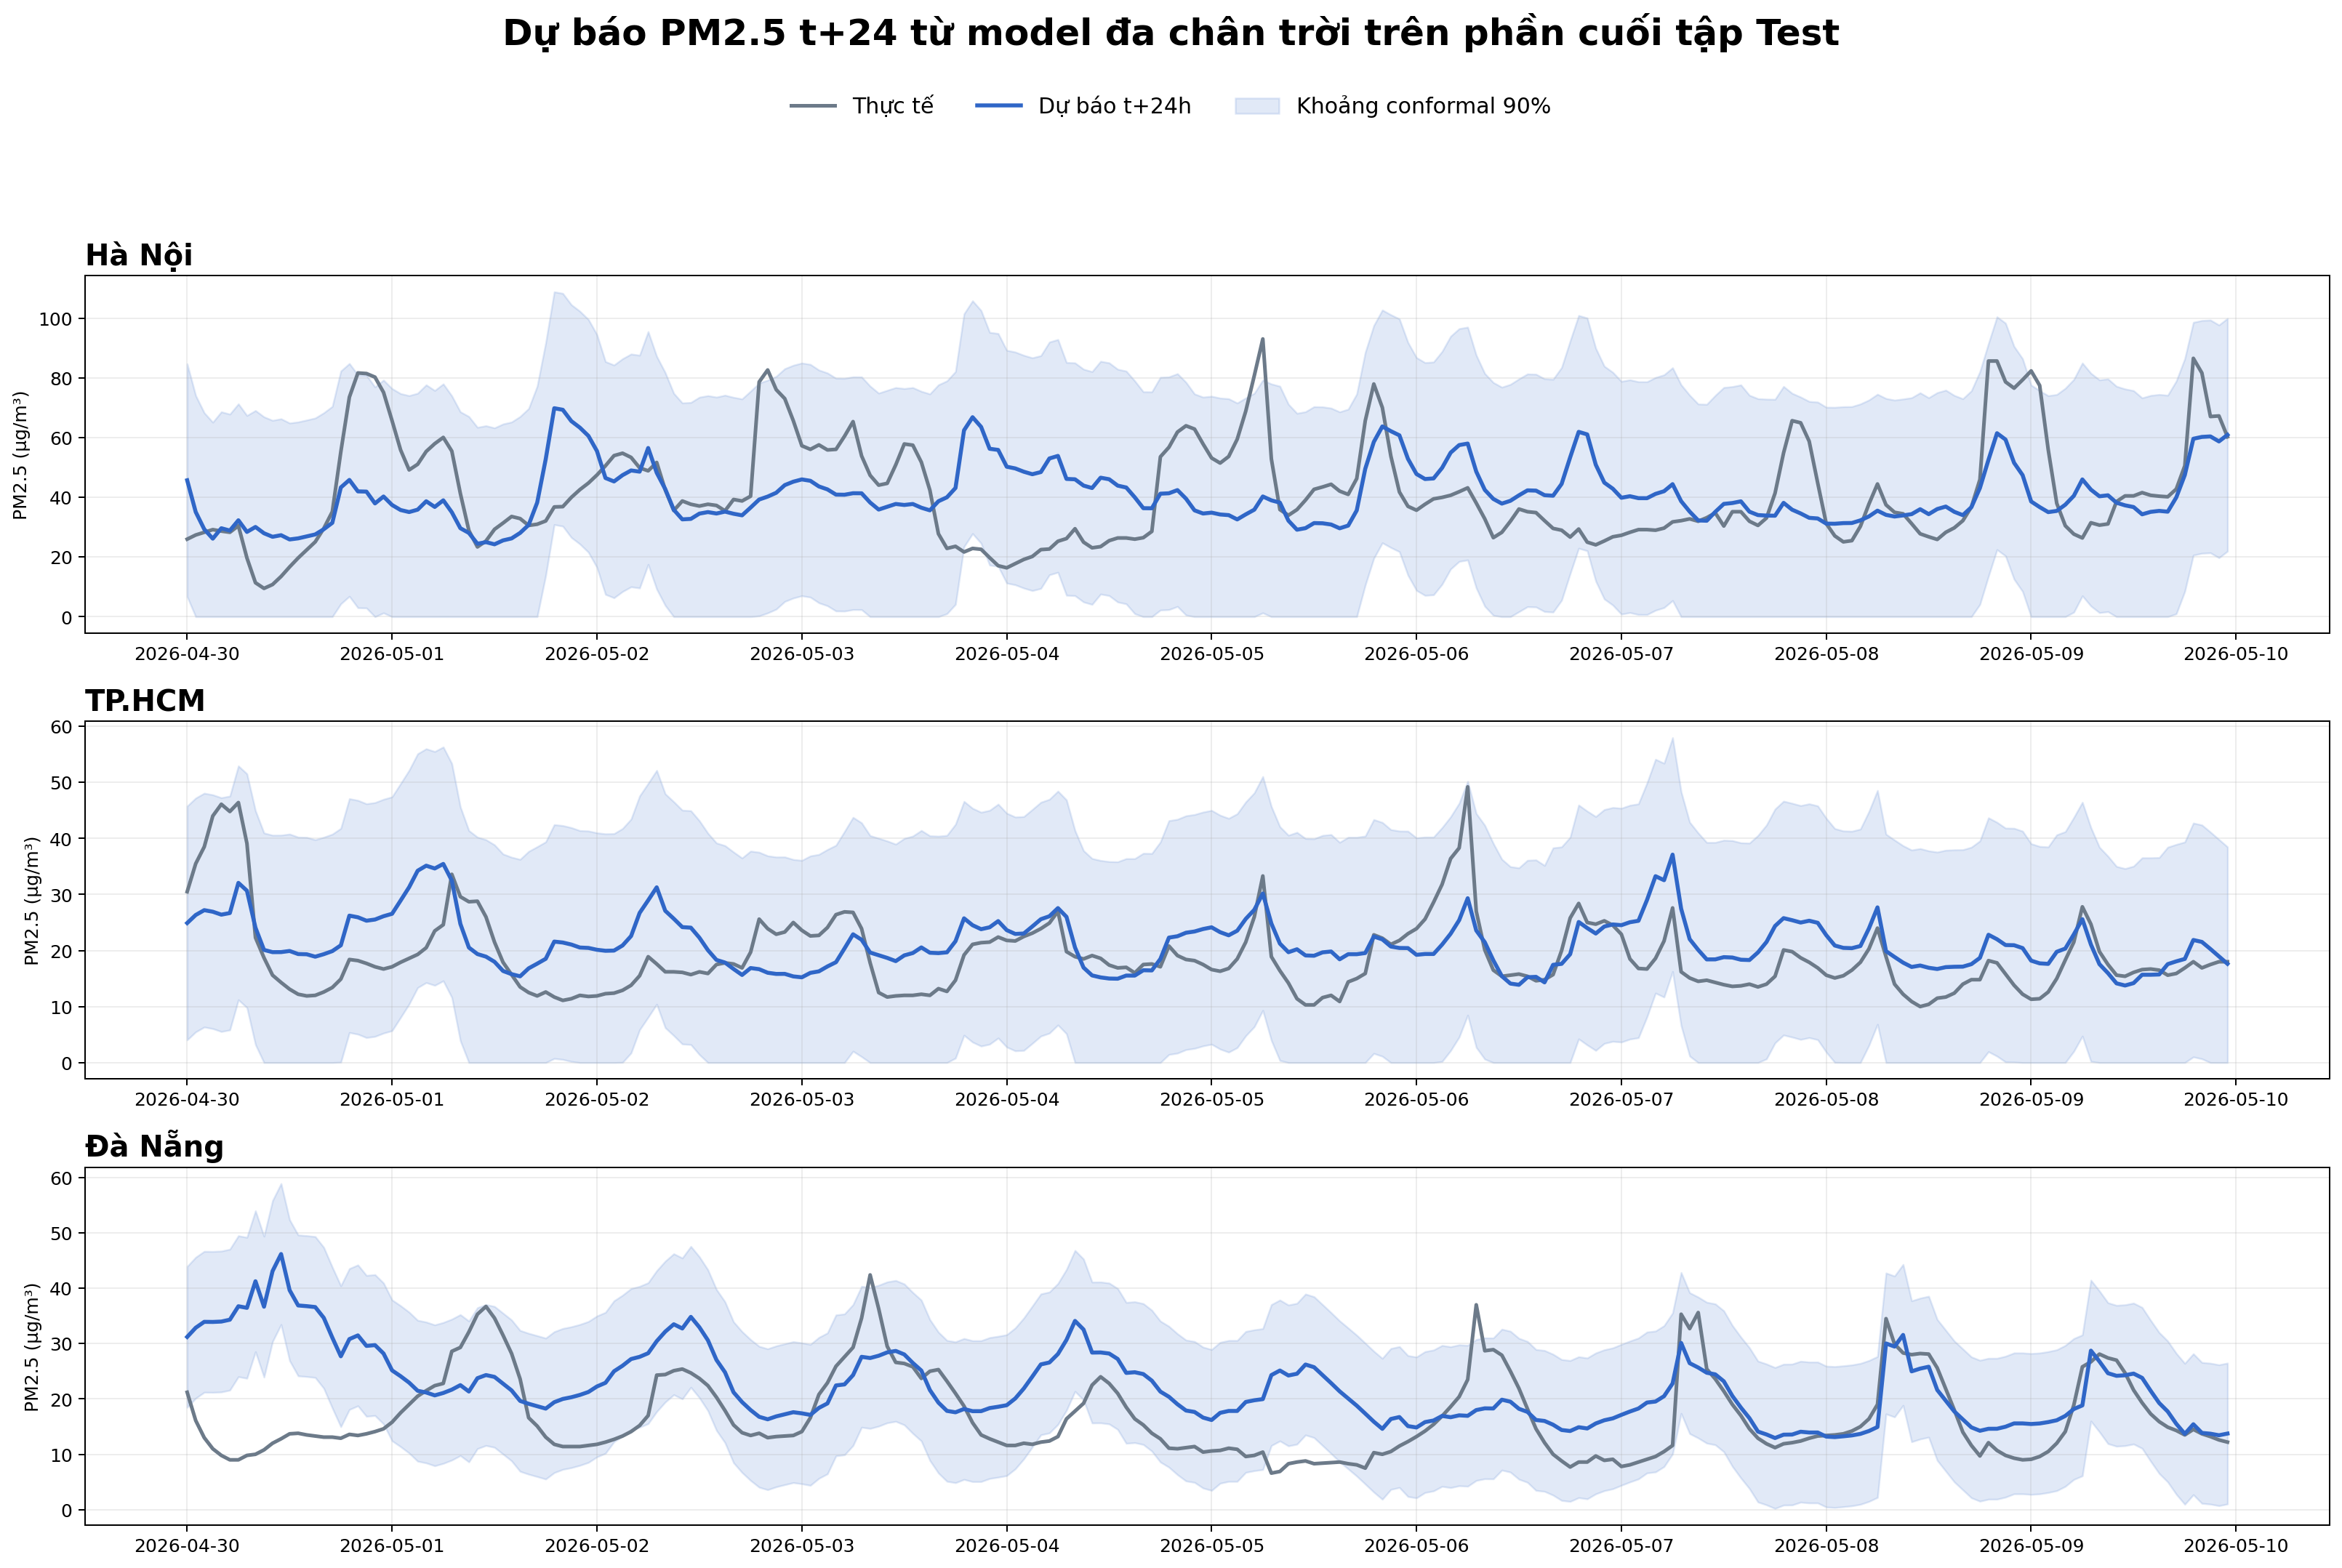
\includegraphics[width=0.98\linewidth]{best_model_test_forecast.png}
\caption{PM2.5 thực tế, dự báo $t+24$ của XGBoost đa chân trời và khoảng conformal 90\% trên 240 giờ cuối của Test tại ba thành phố.}
\label{fig:test-forecast}
\end{figure}

Hình~\ref{fig:test-forecast} cho thấy model bám được nhịp biến động phổ biến nhưng làm trơn một số đỉnh, rõ nhất tại Hà Nội. Khoảng dự báo tại Hà Nội rộng hơn hai thành phố còn lại, phù hợp với RMSE theo thành phố và coverage đã báo cáo. Hình này là bằng chứng trực quan bổ sung; metric ở Bảng~\ref{tab:test} vẫn được tính trên toàn bộ tập Test và toàn bộ 24 horizon.

\subsection{Residual, confusion matrix và lỗi điển hình}
\begin{figure}[H]
\centering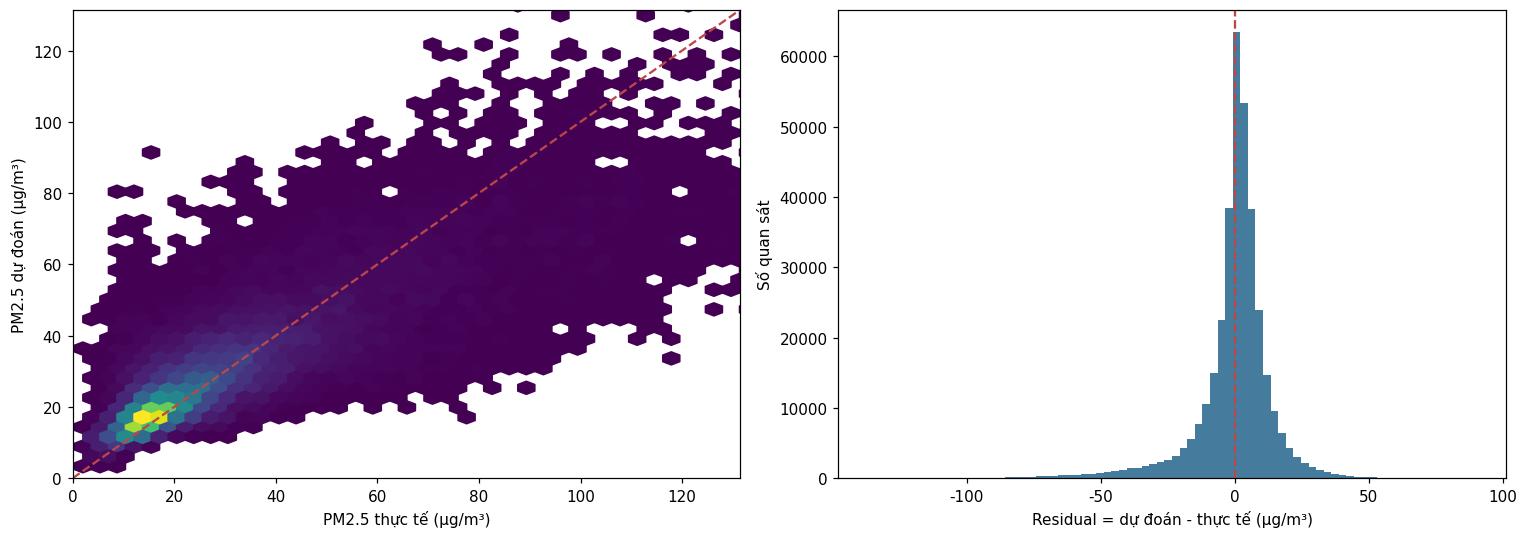
\includegraphics[width=0.96\linewidth]{best_model_residual_analysis.png}
\caption{PM2.5 thực tế--dự đoán và phân phối residual của XGBoost trên Test.}
\label{fig:residual}
\end{figure}

Theo Hình~\ref{fig:residual}, residual tập trung gần 0 ở vùng phổ biến nhưng model làm trơn các đỉnh. Sai số lớn nhất là 136,52 \unitpm tại Hà Nội, horizon 24: thực tế 186,7 nhưng dự báo 50,18. Các lỗi lớn tập trung quanh cùng một đỉnh ngày 25/04/2026, cho thấy một sự kiện ô nhiễm đột ngột ảnh hưởng nhiều origin và horizon.

Ba giả thuyết giải thích được rút ra từ feature và residual. Thứ nhất, đỉnh có thể xuất hiện nhanh hơn các lag và rolling đang quan sát, nên mô hình tiếp tục ngoại suy regime trước đó. Thứ hai, CAMS tại một điểm lưới có thể làm phẳng hoặc lệch thời điểm một sự kiện cục bộ. Thứ ba, squared error tối ưu trung bình có xu hướng kéo dự báo cực trị về vùng dày dữ liệu. Các giả thuyết này phù hợp với bằng chứng lỗi nhưng chưa phải kết luận nhân quả; cần dữ liệu trạm, gió tầng thấp, độ cao lớp biên và nguồn phát thải để kiểm chứng.

\begin{figure}[H]
\centering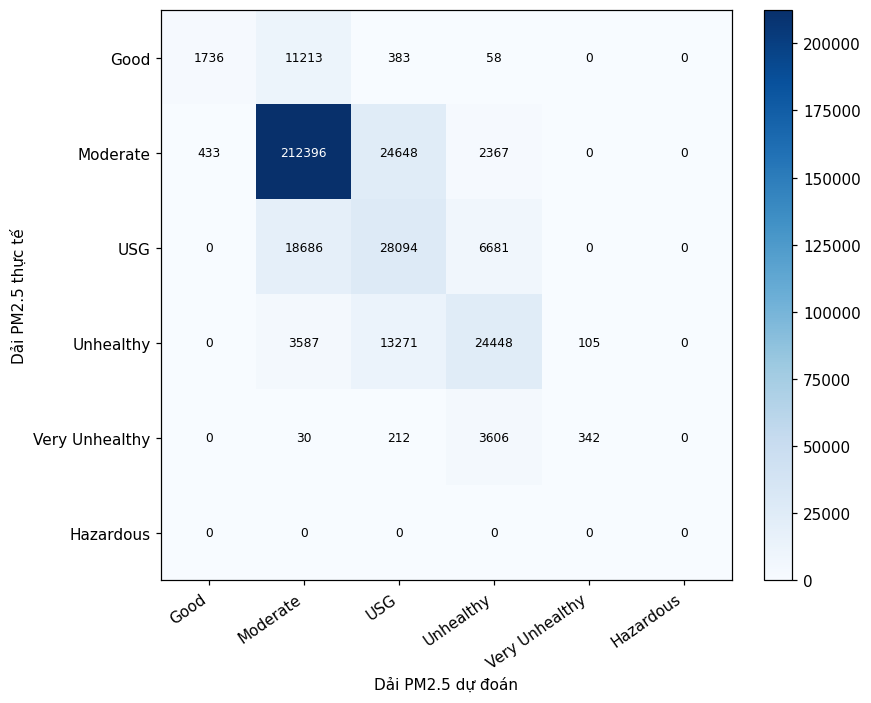
\includegraphics[width=0.67\linewidth]{best_model_confusion_matrix.png}
\caption{Confusion matrix hậu xử lý theo dải PM2.5 do nhóm quy ước; đây không phải bài toán phân loại AQI.}
\label{fig:confusion}
\end{figure}

Hình~\ref{fig:confusion} cho thấy Macro F1 đạt 0,389. Recall của Good là 0,130 và Very Unhealthy là 0,082; không có mẫu Hazardous trong Test. Model nhận diện tốt dải Moderate nhưng yếu ở hai đầu phân phối do mất cân bằng và xu hướng hồi quy về trung bình. Macro F1 thấp không phủ định RMSE 14,01 vì hai metric trả lời hai câu hỏi khác nhau: RMSE đo khoảng cách liên tục, còn F1 phạt việc vượt qua ngưỡng class do nhóm đặt ra. Các hướng cải thiện gồm loss có trọng số theo cực trị, thêm dữ liệu trạm mặt đất và tín hiệu phát thải, hoặc huấn luyện quantile model.

\section{Chương 5: Xây dựng và Triển khai Ứng dụng}
\subsection{Kiến trúc hệ thống}
Hệ thống dùng React/Vite cho frontend, FastAPI cho REST API và artifact \path{model/candidates/xgboost_multihorizon.joblib}. Backend tạo feature profile từ dữ liệu thành phố, chọn regressor theo horizon và trả dự báo điểm, dải sức khỏe cùng khoảng conformal.

Luồng xử lý trong Hình~\ref{fig:architecture} tách giao diện, API và model để mỗi phần có thể kiểm thử độc lập. Frontend chỉ gửi dữ liệu có ý nghĩa với người dùng và không chứa logic ML. Backend chịu trách nhiệm validation request, tải artifact một lần khi khởi động, tái tạo đúng thứ tự 75 feature, chọn regressor $h$, hậu xử lý giá trị âm và thêm metadata. Profile lịch sử và cache cung cấp lag/rolling tự động, vì người dùng thông thường không biết PM2.5 cùng giờ hôm qua hay trung bình 24 giờ.

Artifact không chỉ chứa 24 booster mà còn có danh sách feature, metadata phiên bản, city encoder và bán kính conformal. Cách đóng gói này giảm nguy cơ training--serving skew: nếu frontend thay đổi thứ tự input hoặc backend thiếu một dummy column, request bị từ chối thay vì âm thầm dự báo bằng schema sai. API cũng công khai model version và horizon để kết quả có thể truy vết.

\begin{figure}[H]
\centering
\begin{tikzpicture}[node distance=1.25cm, every node/.style={font=\small}]
\node[draw,rounded corners,fill=blue!8,minimum width=2.6cm,minimum height=0.9cm] (data) {Open-Meteo / CAMS};
\node[draw,rounded corners,fill=green!10,right=of data,minimum width=2.6cm,minimum height=0.9cm] (api) {FastAPI backend};
\node[draw,rounded corners,fill=orange!12,right=of api,minimum width=2.8cm,minimum height=0.9cm] (model) {24 XGBoost models};
\node[draw,rounded corners,fill=purple!10,right=of model,minimum width=2.5cm,minimum height=0.9cm] (ui) {React frontend};
\draw[-{Latex}] (data)--(api); \draw[-{Latex}] (api)--(model); \draw[-{Latex}] (model)--(ui);
\node[draw,rounded corners,fill=gray!10,below=of api,minimum width=3.0cm,minimum height=0.8cm] (cache) {Profile lịch sử và cache};
\draw[-{Latex}] (cache)--(api);
\end{tikzpicture}
\caption{Kiến trúc tích hợp dữ liệu, API, model đa chân trời và giao diện web.}
\label{fig:architecture}
\end{figure}

\subsection{Giao diện và chức năng}
Trang Tổng quan trình bày quan sát mới nhất và lịch sử 24 giờ. Trang Dự báo cho phép chọn thành phố, chọn $t+1$ đến $t+24$, chạy tự động hoặc nhập các biến người dùng hiểu được; lag và rolling được lấy tự động từ profile lịch sử. Trang Phân tích hiển thị xu hướng, còn Mô hình \& Dữ liệu công khai metric, giao thức chọn model và nguồn dữ liệu.

Hai luồng chính ở Hình~\ref{fig:web-main} phục vụ hai nhu cầu khác nhau. Dự báo tự động hoạt động như bản tin thời tiết: hệ thống lấy profile gần nhất và trả đường dự báo 24 giờ. Chế độ nhập kịch bản cho phép thay đổi các biến quan sát dễ hiểu để xem độ nhạy, nhưng giữ feature lịch sử từ thành phố đã chọn; kết quả không được hiểu là can thiệp nhân quả. Các trang bổ sung trong Hình~\ref{fig:web-more} hỗ trợ so sánh thành phố, kiểm tra xu hướng và minh bạch thông tin model.

Màu thành phố được giữ cố định giữa các biểu đồ để tránh người dùng hiểu màu thay đổi là mức nguy hiểm. Dải sức khỏe sử dụng màu riêng cho trạng thái, có text label và giá trị số thay vì chỉ dựa vào màu. Form chọn horizon giới hạn từ 1 đến 24; trạng thái loading, lỗi API và thiếu dữ liệu đều có thông báo. Các trường lag và rolling đã bị loại khỏi form nhập tay, vì hệ thống có thể tính chính xác hơn từ lịch sử.

\begin{table}[H]
\centering\small
\caption{Các API chính của web app}
\label{tab:api}
\begin{tabular}{p{3.4cm}p{2.0cm}p{9.3cm}}
\toprule
Endpoint & Method & Vai trò\\
\midrule
\path{/api/health} & GET & Kiểm tra service, trạng thái model và readiness.\\
\path{/api/model} & GET & Trả phiên bản, model được chọn, metric và phạm vi horizon.\\
\path{/api/forecast} & POST & Nhận thành phố, horizon/kịch bản; trả PM2.5 và khoảng dự báo.\\
\path{/api/predict} & POST & Nhận một kịch bản và trả dự báo tại horizon được chọn.\\
\path{/api/activity-plan} & POST & So sánh tải phơi nhiễm tương đối theo nhóm người dùng và hoạt động.\\
\path{/api/cities} & GET & Trả profile thành phố và timestamp dữ liệu gần nhất.\\
\bottomrule
\end{tabular}
\end{table}

Bảng~\ref{tab:api} là hợp đồng giữa React và FastAPI. Response dự báo cần chứa ít nhất thành phố, origin timestamp, target timestamp, horizon, dự báo điểm, lower/upper bound và class hậu xử lý. Tách health endpoint khỏi forecast giúp nền tảng cloud kiểm tra container mà không chạy suy luận nặng.

\begin{figure}[H]
\centering
\begin{subfigure}{0.49\linewidth}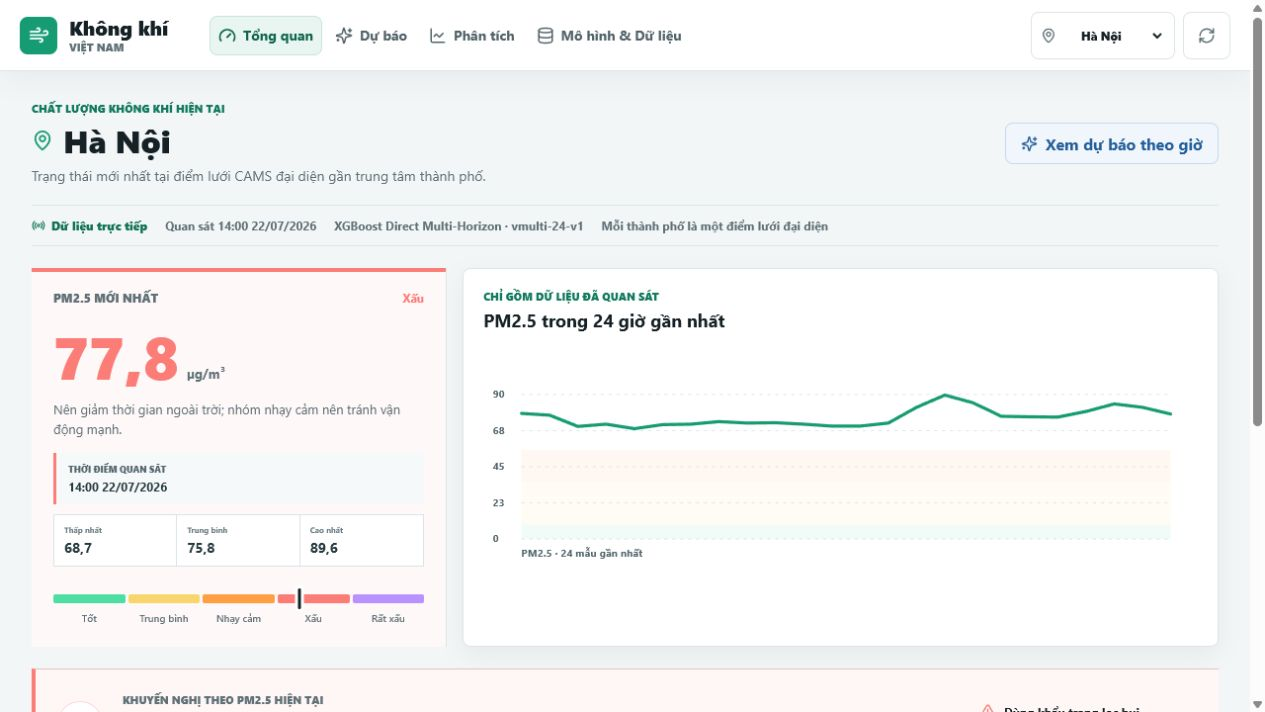
\includegraphics[width=\linewidth]{web_overview.png}\caption{Tổng quan hiện trạng}\end{subfigure}
\begin{subfigure}{0.49\linewidth}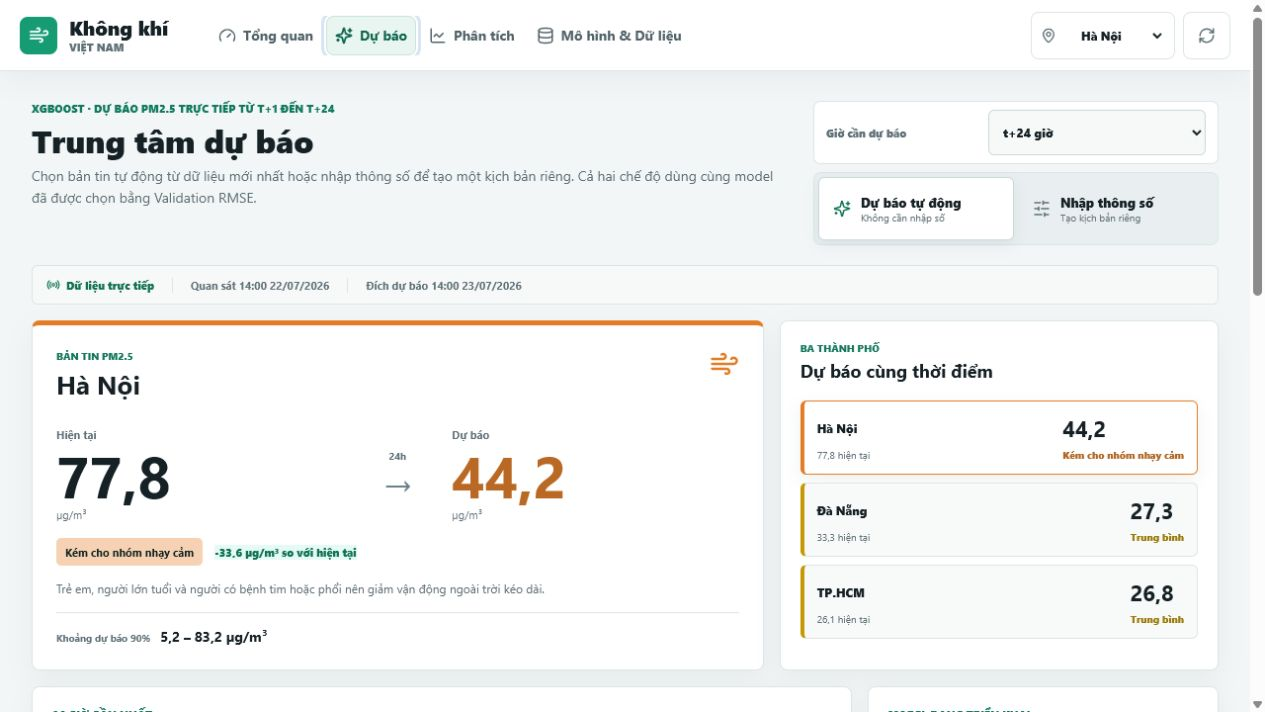
\includegraphics[width=\linewidth]{web_forecast.png}\caption{Dự báo chọn horizon}\end{subfigure}
\caption{Hai luồng chính của ứng dụng web đa chân trời.}
\label{fig:web-main}
\end{figure}

\begin{figure}[H]
\centering
\begin{subfigure}{0.32\linewidth}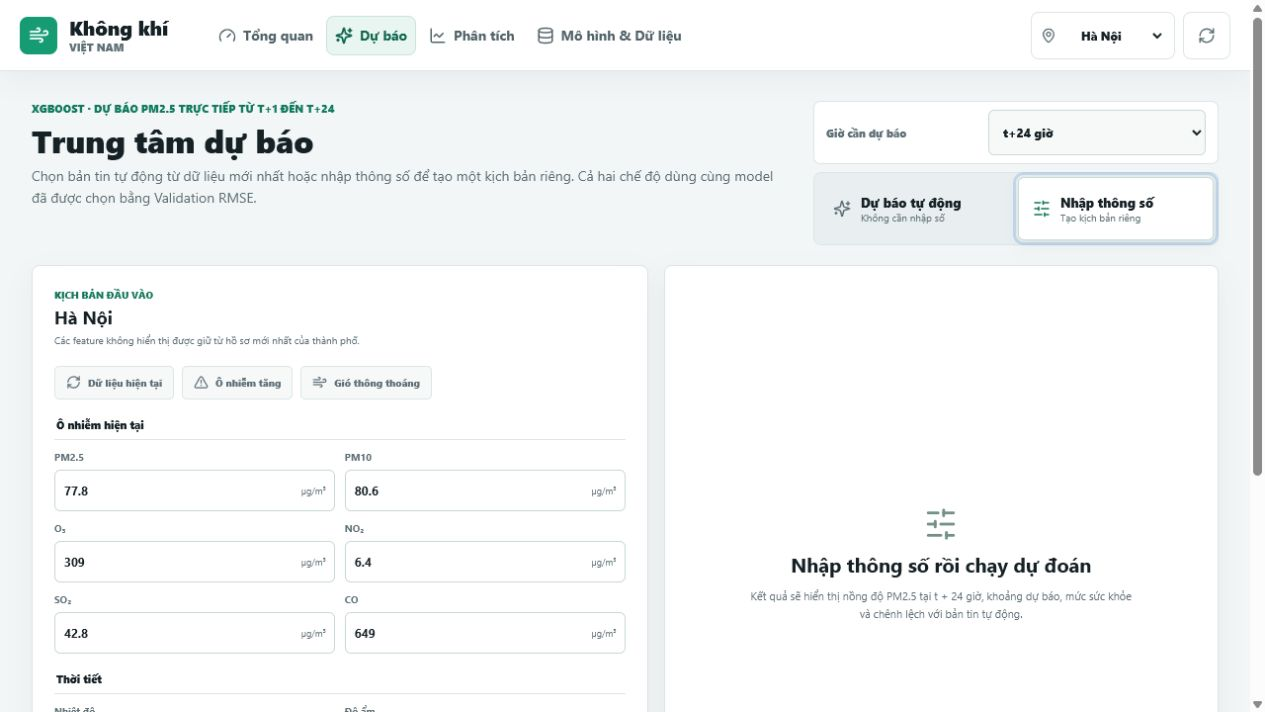
\includegraphics[width=\linewidth]{web_manual_forecast.png}\caption{Nhập kịch bản}\end{subfigure}
\begin{subfigure}{0.32\linewidth}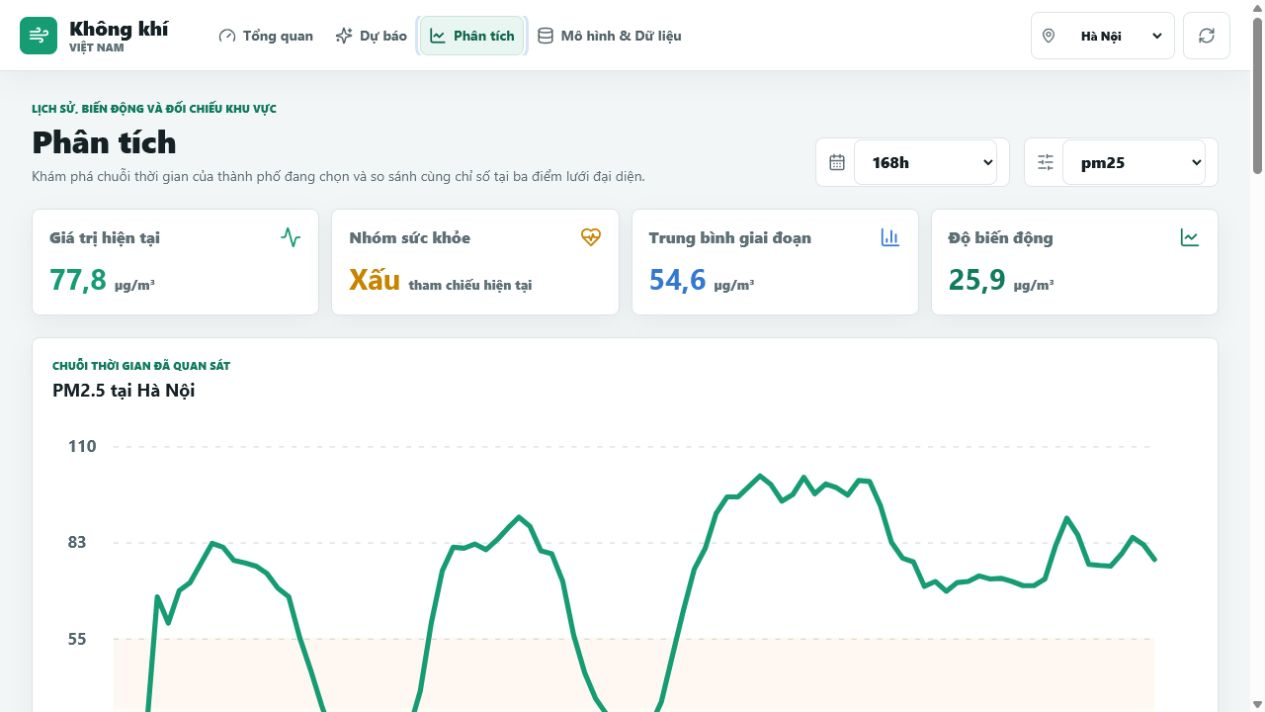
\includegraphics[width=\linewidth]{web_analysis.png}\caption{Phân tích}\end{subfigure}
\begin{subfigure}{0.32\linewidth}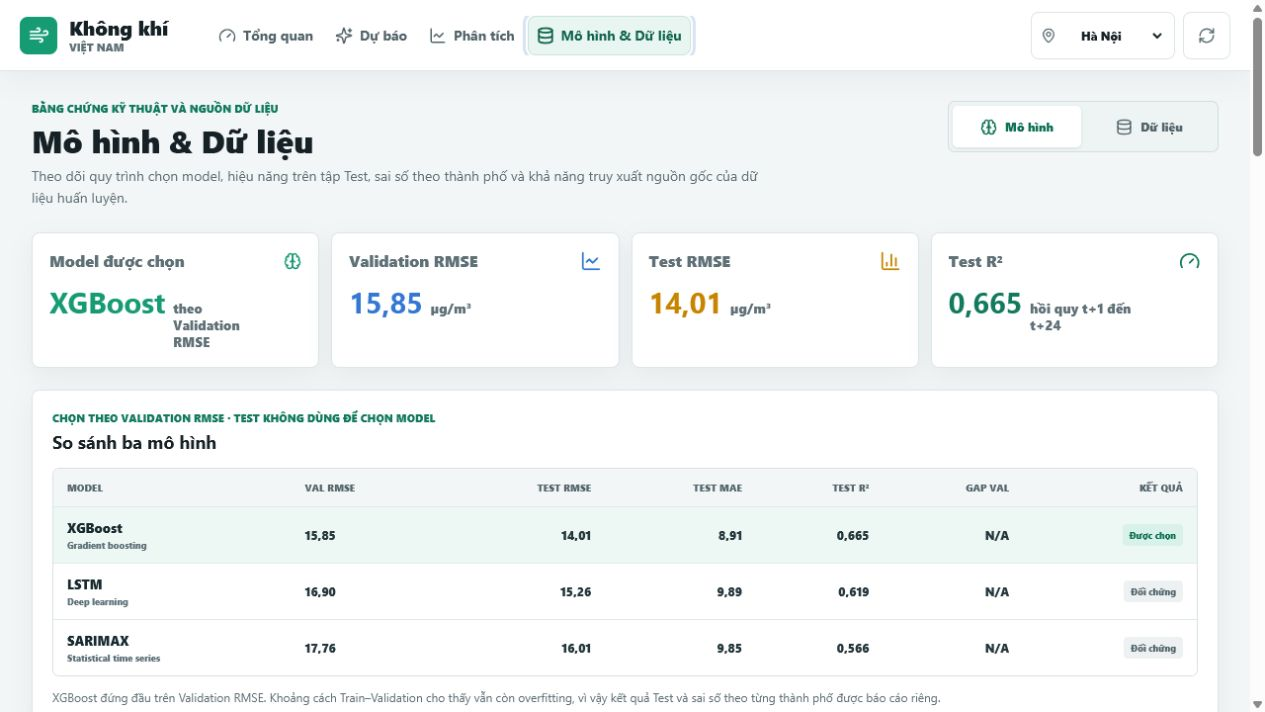
\includegraphics[width=\linewidth]{web_model_data.png}\caption{Mô hình và dữ liệu}\end{subfigure}
\caption{Các chức năng bổ sung của web app.}
\label{fig:web-more}
\end{figure}

\subsection{Chạy local và triển khai cloud}
Các bước chạy local đã được kiểm thử:
\begin{enumerate}
\item Cài Python 3.11 và Node.js; tại \path{web/frontend} chạy \texttt{npm ci} rồi \texttt{npm run build}.
\item Tại thư mục project, chạy \texttt{python -m pip install -r web/requirements-runtime.txt}.
\item Chuyển vào \path{web} và chạy \texttt{python -m uvicorn backend.api:app --host 0.0.0.0 --port 8000}.
\item Mở \url{http://127.0.0.1:8000}; kiểm tra \path{/api/health}, \path{/api/model} và \path{/api/forecast}.
\end{enumerate}
Một Dockerfile đóng gói frontend build và FastAPI trong cùng container, phù hợp Render. Build gồm hai giai đoạn: Node tạo bundle tĩnh, Python cài runtime dependency và copy model/data tối thiểu. Container expose một cổng do biến môi trường \texttt{PORT} điều khiển; FastAPI vừa phục vụ REST API vừa trả frontend đã build. Artifact model và file dữ liệu cần được đưa vào Docker context, không thể chỉ tồn tại ở máy huấn luyện.

Trong cấu trúc source cuối, Render Blueprint đọc \path{render.yaml}, build \path{web/Dockerfile}, kiểm tra readiness tại \path{/api/health} và khởi động FastAPI trên cổng do nền tảng cấp. Bản triển khai đã được nghiệm thu trực tiếp trên Render; URL sử dụng công khai là:

\begin{center}
\url{https://aqi-vietnam-multihorizon.onrender.com}
\end{center}

Health endpoint độc lập:
\begin{center}
\url{https://aqi-vietnam-multihorizon.onrender.com/api/health}
\end{center}

\begin{table}[H]
\centering\small
\caption{Kiểm thử nghiệm thu trực tiếp trên bản cloud ngày 22/07/2026}
\label{tab:cloud-verification}
\begin{tabular}{p{4.0cm}p{2.0cm}p{8.7cm}}
\toprule
Thành phần & Kết quả & Bằng chứng kiểm tra\\
\midrule
Trang React & HTTP 200 & Tải được frontend và chuyển giữa Tổng quan, Dự báo, Phân tích, Mô hình \& Dữ liệu.\\
\path{/api/health} & HTTP 200 & Trạng thái \texttt{ok}; model, data và frontend đều sẵn sàng; artifact có 24 horizon và 75 feature.\\
\path{/api/cities} & HTTP 200 & Trả profile mới nhất cho Hà Nội, TP.HCM và Đà Nẵng.\\
\path{/api/model} & HTTP 200 & Công khai XGBoost Direct Multi-Horizon, phiên bản \texttt{multi-24-v1} và giao thức lựa chọn.\\
\path{/api/forecast} & HTTP 200 & POST cho TP.HCM trả đủ đường dự báo 24 điểm.\\
\path{/api/predict} & HTTP 200 & POST cho TP.HCM tại $t+24$ trả kết quả suy luận hợp lệ.\\
\bottomrule
\end{tabular}
\end{table}

Hình~\ref{fig:cloud-live} được chụp từ chính URL công khai sau khi chọn TP.HCM và horizon $t+24$. Bản tin hiển thị timestamp quan sát, timestamp đích, dự báo điểm, khoảng conformal 90\% và so sánh đồng thời ba thành phố. Đây là bằng chứng ở tầng sản phẩm; bảng kiểm tra endpoint bổ sung bằng chứng ở tầng API và readiness.

\begin{figure}[H]
\centering
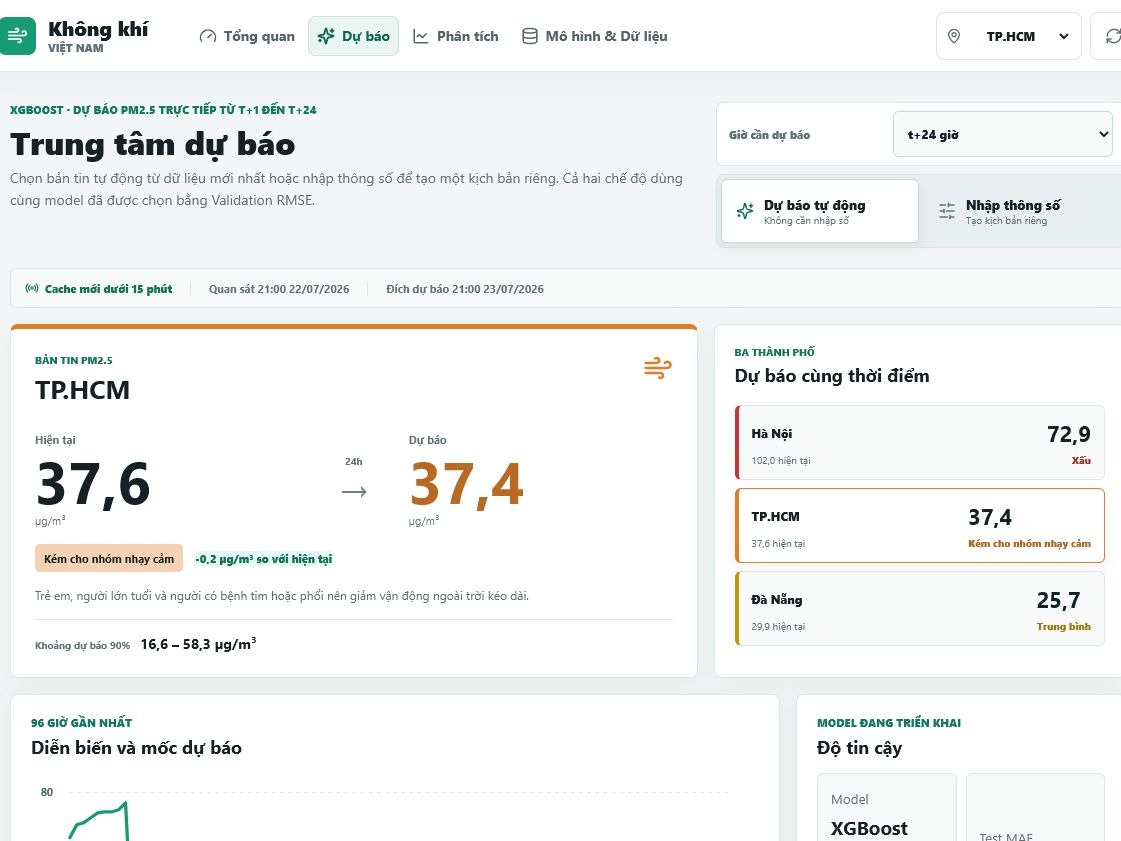
\includegraphics[width=0.98\linewidth]{cloud_deployment_live.png}
\caption{Giao diện dự báo PM2.5 đa chân trời hoạt động trên Render tại URL công khai.}
\label{fig:cloud-live}
\end{figure}

Service dùng gói miễn phí nên có thể bị đưa về trạng thái nghỉ khi không có truy cập; request đầu tiên sau thời gian nghỉ có thể chậm hơn các request tiếp theo. Đây là giới hạn hạ tầng, không phải thời gian suy luận thuần của model. Do đó, nghiệm thu cloud phải dựa trên health endpoint và request dự báo sau khi service đã sẵn sàng, đồng thời không dùng dashboard deploy thay cho kiểm tra HTTP thực tế.

\section{Chương 6: Kết luận}
\subsection{Kết quả đạt được}
Đồ án đã chuyển từ dự báo một mốc $t+24$ sang đường dự báo trực tiếp 24 horizon. Ba model được đánh giá trên cùng target và temporal split. XGBoost thắng năm trên năm khối Validation, đạt Test RMSE 14,01 \unitpm, MAE 8,91 \unitpm và R$^2$ 0,665. Model đã được tích hợp vào web có lựa chọn horizon, hai chế độ dự báo, khoảng conformal và đã triển khai tại URL cloud công khai.

So với mục tiêu ban đầu, hệ thống đã hoàn thành chu trình từ dữ liệu đến sản phẩm: crawl và kiểm tra dữ liệu Việt Nam, EDA, feature engineering chống leakage, huấn luyện ba họ model, lựa chọn bằng Validation theo thời gian, đánh giá Test, phân tích bất định và tích hợp REST API. Giá trị thực tiễn tăng vì người dùng không còn chỉ nhận một con số cuối ngày mà có thể xem diễn biến từng giờ và chọn đúng thời điểm cần quan tâm. Việc công khai metric theo horizon/thành phố và nguồn CAMS giúp sản phẩm không che giấu giới hạn dữ liệu.

\subsection{Hạn chế}
Nguồn CAMS là điểm lưới đại diện, không phải trạm mặt đất; dữ liệu chỉ gồm ba thành phố. Blocked temporal validation kiểm tra candidate đã fit nhưng không refit model ở từng fold. Các khoảng conformal có thể mất coverage khi drift. Model còn đánh giá thấp đỉnh PM2.5, đặc biệt ở Hà Nội và horizon dài. Bản cloud hiện dùng gói miễn phí nên có cold start và chưa có SLA, autoscaling riêng hoặc hệ thống giám sát drift dài hạn.

Ngoài ra, các feature khí tượng tương lai trong dự báo vận hành phải đến từ forecast provider; nếu backend dùng giá trị quan sát tại origin cho toàn bộ horizon thì độ chính xác sẽ giảm khi thời tiết đổi nhanh. Dữ liệu hiện không có giao thông, cháy, công nghiệp, lớp biên khí quyển hoặc trạm tham chiếu để giải thích đỉnh cục bộ. Class hậu xử lý do nhóm quy ước hữu ích cho chẩn đoán nhưng không thay thế quy chuẩn AQI chính thức. Kết quả Test cũng chỉ đại diện cho giai đoạn 17/10/2025--08/05/2026; chưa đủ để khẳng định ổn định nhiều năm.

\subsection{Hướng phát triển}
Mở rộng dữ liệu trạm quan trắc, thêm mưa vệ tinh, giao thông và nguồn phát thải; thử quantile XGBoost, Temporal Fusion Transformer hoặc N-BEATS; dùng weighted loss cho cực trị; triển khai rolling recalibration conformal; giám sát drift và tái huấn luyện theo lịch. Với strict rolling-origin CV, cần refit cả ba mô hình trên từng fold bằng ngân sách tính toán được kiểm soát.

Ở tầng sản phẩm, cần lưu prediction cùng ground truth khi timestamp tương lai đã đến để tạo dashboard giám sát MAE/RMSE theo horizon, thành phố và tuần. Trigger cảnh báo nên dựa trên cả dự báo điểm lẫn xác suất/khoảng bất định. Khi coverage hoặc residual drift vượt ngưỡng, pipeline sẽ crawl bổ sung, kiểm tra chất lượng, tái huấn luyện candidate, chạy temporal backtest và chỉ promote artifact mới nếu vượt model hiện hành. Quy trình này biến web demo thành hệ thống học máy có vòng đời vận hành rõ ràng.

\begin{thebibliography}{9}
\bibitem{tashman} Tashman, L. J. (2000). Out-of-sample tests of forecasting accuracy: an analysis and review. \textit{International Journal of Forecasting}, 16(4), 437--450.
\bibitem{xgb} Chen, T., \& Guestrin, C. (2016). XGBoost: A Scalable Tree Boosting System. \textit{Proceedings of KDD}.
\bibitem{lstm} Hochreiter, S., \& Schmidhuber, J. (1997). Long Short-Term Memory. \textit{Neural Computation}, 9(8), 1735--1780.
\bibitem{sarimax} Box, G. E. P., Jenkins, G. M., Reinsel, G. C., \& Ljung, G. M. (2015). \textit{Time Series Analysis: Forecasting and Control}. Wiley.
\bibitem{conformal} Angelopoulos, A. N., \& Bates, S. (2023). Conformal prediction: A gentle introduction. \textit{Foundations and Trends in Machine Learning}, 16(4), 494--591.
\bibitem{openmeteo} Open-Meteo. Air Quality API and Historical Weather API. \url{https://open-meteo.com/}.
\end{thebibliography}

\end{document}
